%%%%%%%%%%%%%%%%%%%%%%%%%%%%%%%%%%%%%%%%%%%%%%%%%%%%%%%%%%%%%%%%%%%%%%
%%  dissertation.tex, to be compiled with pdfLaTeX.		     %
%%  19 January 2023	Version 5				     %
%%%%%%%%%%%%%%%%%%%%%%%%%%%%%%%%%%%%%%%%%%%%%%%%%%%%%%%%%%%%%%%%%%%%%%
%%  Writing a Doctoral Dissertation with LaTeX at		     %
%%	the University of Texas at Austin			     %
%%  (Modify this template for your own dissertation.)	     %
%%%%%%%%%%%%%%%%%%%%%%%%%%%%%%%%%%%%%%%%%%%%%%%%%%%%%%%%%%%%%%%%%%%%%%

\documentclass[letterpaper,12pt]{report}	% The documentclass must be ``report''.

% Includes the utformat.sty file, but also additional packages and some commands.
% See `structural/preamble.tex`.

\usepackage[authoryear, round]{natbib}
\usepackage{styles/utformat}  		% Package style file for UT ETDs.


%%%%%%%%%%%%%%%%%%%%%%%%%%%%%%%%%%%%%%%%%%%%%%%%%%%%%%%%%%%%%%%%%%%%%%
% Optional packages used for this template. If you don't
% need a capability in your document, feel free to comment out/remove
% the package usage command.
%%%%%%%%%%%%%%%%%%%%%%%%%%%%%%%%%%%%%%%%%%%%%%%%%%%%%%%%%%%%%%%%%%%%%%
\usepackage[T1]{fontenc}
\usepackage[utf8]{inputenc}
\usepackage{pdflscape}
\usepackage{layout}
\usepackage{graphicx}
\usepackage{amsmath,amsthm,amsfonts,amscd}
\usepackage{unicode-math}
\usepackage{eucal} 	 
\usepackage{verbatim}    
\usepackage{styles/citesort}     
\usepackage{algorithm}
\usepackage{bibentry}
\usepackage{algorithmic}
\usepackage{xcolor}
\usepackage{markdown}
\usepackage{booktabs}
\usepackage{url}

\usepackage{multirow}
\usepackage{makecell}
\usepackage{tabularx}
\usepackage{bbm}% Allows good typesetting of web URLs.
\usepackage{mathtools}
\usepackage{hyperref}
\hypersetup{
    colorlinks,
    breaklinks,
    linkcolor=black,
    urlcolor=AmmaBlue,
    citecolor=AmmaBlue,
    filecolor=AmmaBlue
}


% Typography
\setmainfont[Numbers={Lowercase,Proportional}, Contextuals=Alternate]{Century Supra B}
\newcommand\liningfont{\addfontfeatures{Numbers={Uppercase, Proportional}}}
\newfontfamily{\rmsc}{Century Supra B Caps}[Letters=UppercaseSmallCaps, LetterSpace=5, Numbers={Lowercase,Proportional}]
\newfontfamily{\rmcs}{Century Supra B Caps}[Letters=Uppercase, LetterSpace=5, Numbers={Uppercase,Proportional}]

% IPA, monospace, and math fonts
\setmonofont[Scale=0.9]{Triplicate A}
\setmathfont[Path=/Users/venkat/Library/Fonts/, Extension=.otf,Scale=0.9,Ligatures=TeX, BoldFont=XCharter-Bold,
    ItalicFont=XCharter-Italic, Numbers={Uppercase,Monospaced}]{XCharter-Roman}

% Oldstyle tabular numbers inside tabular environment
\AtBeginEnvironment{tabular}{\addfontfeatures{Numbers={Uppercase, Monospaced}}}
\AtBeginEnvironment{tikzpicture}{\addfontfeatures{Numbers={Uppercase, Monospaced}}\small}
\renewcommand{\theequation}{ {\addfontfeatures{Numbers={Uppercase, Monospaced}}\small\arabic{equation}}}

% Custom Blue
\definecolor{AmmaBlue}{HTML}{0366D6}
\definecolor{TolIndigo}{HTML}{332288}
\definecolor{TolCyan}{HTML}{88CCEE}
\definecolor{TolTeal}{HTML}{44AA99}
\definecolor{TolGreen}{HTML}{117733}
\definecolor{TolOlive}{HTML}{999933}
\definecolor{TolSand}{HTML}{DDCC77}
\definecolor{TolRose}{HTML}{CC6677}
\definecolor{TolWine}{HTML}{882255}
\definecolor{TolPurple}{HTML}{AA4499}
\definecolor{TolPaleGrey}{HTML}{DDDDDD}

\usepackage{linguex}
\usepackage{soul}
\usepackage{pgfplots}
\pgfplotsset{compat=newest}
\usetikzlibrary{shapes,arrows}

%%%%%%%%%%%%%%%%%%%%%%%%%%%%%%
% Default is one-and-a-half spacing. Double is also permitted.%
%%%%%%%%%%%%%%%%%%%%%%%%%%%%%%
\oneandonehalfspacing
% \doublespacing

% Strong widow and orphan control - avoid any widows and orphans
\clubpenalty10000
\widowpenalty10000

% French Spacing - single spacing between sentences
\frenchspacing

%%%%%%%%%%%%%%%%%%%%%%%%%%%%%%%%%%%%%%%%%%%%%%%%%%%%%%%%%%%%%%%%%%%%%%
%	Some math support.					     %
%%%%%%%%%%%%%%%%%%%%%%%%%%%%%%%%%%%%%%%%%%%%%%%%%%%%%%%%%%%%%%%%%%%%%%
%
%	Theorem environments (these need the amsthm package)
%
%% \theoremstyle{plain} %% This is the default
% 
% \newtheorem{thm}{Theorem}[chapter]
% \newtheorem{cor}[thm]{Corollary}
% \newtheorem{lem}[thm]{Lemma}
% \newtheorem{prop}[thm]{Proposition}
% \newtheorem{ax}{Axiom}
% 
% \theoremstyle{definition}
% \newtheorem{defn}{Definition}[chapter]
% 
% \theoremstyle{remark}
% \newtheorem{rem}{Remark}[chapter]
% \newtheorem*{notation}{Notation}

%\numberwithin{equation}{section}


%%%%%%%%%%%%%%%%%%%%%%%%%%%%%%%%%%%%%%%%%%%%%%%%%%%%%%%%%%%%%%%%%%%%%%
%	Macros.							     %
%%%%%%%%%%%%%%%%%%%%%%%%%%%%%%%%%%%%%%%%%%%%%%%%%%%%%%%%%%%%%%%%%%%%%%
%
%	Here some macros that are needed in this document:


\newcommand{\latexe}{{\LaTeX\kern.125em2%
                      \lower.5ex\hbox{$\varepsilon$}}}

\newcommand{\amslatex}{\AmS-\LaTeX{}}

\chardef\bslash=`\\	% \bslash makes a backslash (in tt fonts)
			%	p. 424, TeXbook

\newcommand{\cn}[1]{\texttt{\bslash #1}}

\makeatletter		% Starts section where @ is considered a letter
			% and thus may be used in commands.
\def\square{\RIfM@\bgroup\else$\bgroup\aftergroup$\fi
  \vcenter{\hrule\hbox{\vrule\@height.6em\kern.6em\vrule}%
                                              \hrule}\egroup}
\makeatother		% Ends sections where @ is considered a letter.
			% Now @ cannot be used in commands.

\nobibliography*


% These values determine the numbering within the text and Table of Contents.
\setcounter{secnumdepth}{3}    % Number subsections in the chapters.
\setcounter{tocdepth}{1} % include subsections in the Table of Contents
  

% Important! Need to update the information in `structural/about.tex`!
\author{Venkata Subrahmanyan Govindarajan}  	% Required

\address{venkatasg@utexas.edu}  % Required

\title{Modeling Intergroup Bias in Online Conversation} % Required

%%%%%%%%%%%%%%%%%%%%%%%%%%%%%%%%%%%%%%%%%%%%%%%%%%%%%%%%%%%%%%%%%%%%%%
% NOTICE: The total number of supervisors and other members %%%%%%%%%%
%%%%%%%%%%%%%%% MUST be seven (7) or less! If you put in more, %%%%%%%
%%%%%%%%%%%%%%% they are put on the page after the Committee %%%%%%%%%
%%%%%%%%%%%%%%% Certification of Approved Version page. %%%%%%%%%%%%%%
%%%%%%%%%%%%%%%%%%%%%%%%%%%%%%%%%%%%%%%%%%%%%%%%%%%%%%%%%%%%%%%%%%%%%%

%%%%%%%%%%%%%%%%%%%%%%%%%%%%%%%%%%%%%%%%%%%%%%%%%%%%%%%%%%%%%%%%%%%%%%
%
% Enter names of the supervisor and co-supervisor(s), if any,
% of your dissertation committee. Put one name per line with
% the name in square brackets. The name on the last line, however,
% must be in curly braces. The name first listed (either in square
% brackets or curly braces) will be the "Supervisor."
%
% If you have only one supervisor, the entry below will read:
%
	% \supervisor
	% 	{Supervisor's Name}
%
% TECH NOTE: Maximum three supervisors. Minimum one supervisor.
% NOTE: The Office of Graduate Studies will accept only two supervisors!
%
%
\supervisor[Junyi Jessy Li]
	{David Beaver}

%%%%%%%%%%%%%%%%%%%%%%%%%%%%%%%%%%%%%%%%%%%%%%%%%%%%%%%%%%%%%%%%%%%%%%
%
% Enter names of the other (non-supervisor) members(s) of your
% committee. Put one name per line with the name
% in square brackets. The name on the last line, however, must
% be in curly braces.
%
% To not include any additional members, use
%
% \committeemembers{}
%
% NOTE: Maximum six other members. Minimum zero other members.
% NOTE: The Office of Graduate Studies may restrict you to a total
%	of six committee members.
%
%
\committeemembers
	[Kyle Mahowald]
	[Malihe Alikhani]
    {}
 

% Please update your degree and degree abbreviation here, if needed.
% \degree{Doctor of Philosophy}
\degree{Doctor of Philosophy}
\degreeabbr{PhD} 
% See the Catalog for the current list.
% catalog.utexas.edu/graduate/graduate-study/graduate-degrees/

% Uncomment ONLY the line below that corresponds to the type of document you are writing.

\dissertation


% Define block styles
\tikzstyle{block} = [rectangle, draw, fill=TolSand!80, text centered, rounded corners, minimum height=2em]
\tikzstyle{tweet} = [rectangle, draw, fill=TolCyan!60,
    text width=30em, text centered, rounded corners, minimum height=0.5em]
\tikzstyle{line} = [draw, -latex']
\tikzstyle{cloud} = [draw, ellipse,fill=TolRose!70, node distance=0.5cm,minimum height=1em]

\begin{document}

% See `structural/body.tex` for updating/adding/removing content.
% This is the body of your document. You may copy-paste it into your main document
% (dissertation.tex, masterreport.tex, masterthesis.tex, treatise.tex), or edit it here.


\copyrightpage  % Produces the copyright page. Optional.

\commcertpage   % Produces the Committee Certification
			%   of Approved Version page (doctoral)
			%   or Signature page (masters).
			%		20 Mar 2002	cwm
                % Required.

\titlepage      % Produces the title page. Required.


%%%%%%%%%%%%%%%%%%%%%%%%%%%%%%%%%%%%%%%%%%%%%%%%%%%%%%%%%%%%%%%%%%%%%%
% Dedication and/or epigraph are optional, but must occur here.      %
%%%%%%%%%%%%%%%%%%%%%%%%%%%%%%%%%%%%%%%%%%%%%%%%%%%%%%%%%%%%%%%%%%%%%%
\begin{dedication}		% Optional
\begin{center}
    To my mother and father.
\end{center}
\end{dedication}

\begin{epigraph}		% Optional
    \begin{center}
        \textit{Machine learning is like money laundering for bias.  It’s a clean, mathematical apparatus that gives the status quo the aura of logical inevitability. The numbers don’t lie.}
        \\\hspace{4em}---Maciej Ceglowski, \href{https://idlewords.com/talks/sase_panel.htm}{The Moral Economy of Tech}
    \end{center}
\end{epigraph}

%%%%%%%%%%%%%%%%%%%%%%%%%%%%%%%%%%%%%%%%%%%%%%%%%%%%%%%%%%%%%%%%%%%%%%
% Acknowledgements and/or preface are optional, but must occur here. %
%%%%%%%%%%%%%%%%%%%%%%%%%%%%%%%%%%%%%%%%%%%%%%%%%%%%%%%%%%%%%%%%%%%%%%
\begin{acknowledgments}		% Optional
    This dissertation would not have been possible without the support of many people. I would like to thank my advisors Jessy, David, Kyle and Malihe, for their generosity over the last five years. They have always set aside their valuable time to talk to me about my progress, successes and failures. Thank you deeply.
    
    I owe a debt of gratitude to Matianyu (Yuki) Zang, my collaborator over the last year, whose work on data curation and preprocessing has been invaluable. 
    
    My favorite activity in my PhD has been the research seminars, particularly the Computational Linguistics seminar, that I have attended weekly since Fall 2019. The conversations and arguments over research papers and projects with Katrin, Gabriella, Yejin, Juan Diego, Yating, Will, Hongli, Kanishka and many other researchers have taught me what it means to do research and be an academic, and made me a betteer one for it. Thank you for your feedback and thoughts on all my talks over the years.
    
    The last five years have been easier to bear with a close group of friends --- Benny, Gus, Hunter, and Ethan who I co-habited with through the beginning of the pandemic, and many years into it. Blake, Bryan and Erin for all those nights spent eating, drinking, at trivia, and commiserating as we navigated grad school. Sam, for choosing me as his side-kick with SXSemantics, and for being there for me when I needed community the most. Karoline, for a loving relationship that I will always cherish. Thank you all for welcoming me in, and for accepting all of me.
    
    Everything in the end comes back to my mother and father, who have wished nothing else but for me to study and learn, and built opportunities for me that were never afforded to them. I am indebted to them for the opportunity to spend five years trying to understand this world a little bit more.
\end{acknowledgments}

% The abstract is required. Note the use of ``utabstract'' instead of
% ``abstract''! This was necessary to fix a page numbering problem.
% The abstract heading is generated automatically.
% Do NOT use \begin{abstract} ... \end{abstract}.
%
\utabstract
Social bias in language is generally studied by identifying undesirable language use towards a specific demographic group, but we can enrich our understanding of communication by re-framing bias as \emph{differences in behavior situated in social relationships} --- specifically, the intergroup relationship between the speaker and target reference of an utterance. This dissertation aims to understand the nature of systematic variation between in-group and out-group speech --- the intergroup bias. Chapter~\ref{chapter:twitter} describes systematic interactions between intergroup bias and interpersonal emotion, and finds that learned neural models can learn to classify the intergroup relationship in tweets with information about the speaker and target masked, out-performing expert annotators. To decipher what human-interpretable linguistic features are learned by these models, Chapter~\ref{chapter:probing} describes probing experiments to understand if two pragmatic features --- affect and specificity --- are \emph{used} by these models in differentiating in-group from out-group utterances. While affect and specificity have directional impacts on model prediction that align with our intuitions (positive affect utterances are more likely to be in-group), we found no interaction between these two variables, as we hypothesized generalizing from the Linguistic Intergroup Bias. Experiments up until this point also demonstrated the need for interpersonal language use \emph{grounded} in non-linguistic world-state. To address this, Chapter~\ref{chapter:football} investigates online comments from live game threads on forums (subreddits) dedicated to individual NFL teams. We find systematic linear relationships between the \emph{form of referent} used to describe in-group and out-group teams, and the win probability for the in-group (game state) at the time of utterance. The better the state-of-the-world for the in-group, fans refer to the in-group less and the out-group more. Fans are also more likely to abstract away from events of the game and not refer to the in-group or out-group at all, choosing instead to express excitement, the more likely the in-group is to win. State-of-the-world as expressed in the win probability for the in-group turns out to be a well calibrated metric for intergroup bias, as evidenced by the linear relationships between several referent forms and win probability for the in-group. Data-driven analysis and experimentation with modern NLP tools in this dissertation thus revealed a form of intergroup bias ignored in previous literature, and outlines a promising picture of utilizing statistical information processing paired with careful data curation and analysis to understand subtle changes in human social behavior
    % this includes the text from `abstract.tex`

\tableofcontents   % Table of Contents will be automatically
                   % generated and placed here. Required.

\listoftables      % Optional.
\listoffigures     % Optional.

%%%%%%%%%%%%%%%%%%%%%%%%%%%%%%%%%%%%%%%%%%%%%%%%%%%%%%%%%%%%%%%%%%%%%%
% Actual text starts here.					     %
%%%%%%%%%%%%%%%%%%%%%%%%%%%%%%%%%%%%%%%%%%%%%%%%%%%%%%%%%%%%%%%%%%%%%%
%
% Including external files for each chapter makes this document simpler,
% makes each chapter simpler, and allows for generating test documents
% with as few as zero chapters (by commenting out the include statements).
% Can even change the chapter order by merely interchanging the order
% of the include statements (something past contributors found helpful in their own
% dissertations =) ).
%

\chapter{Introducing intergroup bias}
\label{chapter:intro}

Currently, most work studying bias in NLP situates bias as negative or pejorative language use towards an individual or group based on traits like race, gender, etc~\citep{kaneko-bollegala-2019-gender, sheng-etal-2019-woman, sap-etal-2020-social, webson-etal-2020-undocumented, Pryzant_DiehlMartinez_Dass_Kurohashi_Jurafsky_Yang_2020, sheng-etal-2020-towards}.  While these approaches greatly advance our understanding of bias in language and its impact and mitigation in NLP, focusing on specific demographic dimensions or an individual's intent is limiting and not always practical. Research in psychology and social science suggests a different perspective. Bias can be seen as a relationship between people and groups, situated in context~\citep{van2009society}; as such, bias refers to differences in behavior (in this case language use) as a result of differences in the relationship between speaker and target. The language we produce is biased in one way or another, whether we intend to or not, and whether that bias is positive, negative, or not clearly associated with any valuation~\citep{beaver2018toward}.

So how do we study bias from this perspective? By accepting that the language we produce is biased, and is dependent on our social identity and relationships to the people we talk about (and to), we can focus on various aspects of modeling the subtle influence of social identity relationships on our linguistic production, as well as how language shapes and informs social identity in turn~\citep{eckert2012three}. One such form of social meaning~\citep{Hall-Lew_Moore_Podesva_2021,beltrama2020social}, that will be the focus of this dissertation is \textbf{intergroup bias}. The next section introduces the psycho-linguistic literature behind studies of the Linguistic Intergroup Bias, and its deficiencies that makes drawing inferences on social communication more broadly hard. By focusing on data-driven studies of in-group versus out-group speech in the wild, this dissertation aspires holistic understanding of how intergroup social differences has a bearing on the form, and meaning, of the language we produce.

\section{The Linguistic Intergroup Bias}
\label{sec:intro-lib}

The Linguistic Intergroup Bias hypothesis tries to explain why stereotypes persist, and how they are transmitted sub-consciously in daily conversation. In an intergroup context, and focusing on actions that are considered stereotypical for a group, socially desirable in-group behaviors and undesirable out-group behaviors are encoded at a higher level of \textbf{abstraction}, whereas socially undesirable in-group behaviors and desirable in-group behaviors are encoded at a lower level of abstraction (described in Table~\ref{tab:lib}. A crucial underpinning of the theory is the Linguistic Category Model~\citep{semin_cognitive_1988}.

\begin{table}[t]
    \centering
    \begin{tabular}{lll}
     \toprule
        \textbf{} & \textbf{In-group} & \textbf{Out-group} \\ \midrule
        socially desirable & abstract & concrete \\ \midrule
        socially undesirable & concrete & abstract \\ 
    \bottomrule
    \end{tabular}
    \caption{Predicted language variation in the LIB.}
    \label{tab:lib}
\end{table}


The Linguistic Category Model classifies predicates (words that can be used to describe people; like adjectives and verbs) on a scale of increasing abstraction -- from verbs that are most concrete, to verbs that are less concrete, to adjectives that are most abstract. Abstract words (and thus statements) are taken to imply greater {\scshape temporal stability} and revealing of the character of a referent than their concrete counterparts. This provides an explanation for the persistence of bias and stereotypes through LIB -- people tend to use abstract statements to talk about desirable in-group and undesirable out-group behaviors since they are \textbf{potentially more informative of the referent} (that is, indicative of future behavior). Consider the following utterances regarding a subject \textit{Johnson} (examples taken from \citet{gorham_news_2006}):

\ex. \label{ex:exs} \a. The man police want to talk to probably hit the victims.\label{ex:dav}
     \b. The man police want to talk to probably hurt the victims.\label{ex:iav}
     \b. The man police want to talk to probably hated the victims.\label{ex:sv}
     \b. The man police want to talk to is probably violent .\label{ex:adj}
     
\textit{hurt} in \ref{ex:dav} is a direct action verb; \textit{hurt} in \ref{ex:iav} is an interpretive action verb; \textit{hated} in \ref{ex:sv} is a stative and; \textit{violent} is an adjective. Moving from \ref{ex:dav} to \ref{ex:adj}, one can see how the information about the subject increases, while the information regarding a specific situation \textit{decreases}. Thus, the \emph{abstractness} of predicates increases from \ref{ex:dav} to \ref{ex:adj} according to the LCM.

The LIB uses the LCM ladder of abstraction to predict linguistic behavior: a speaker is more likely to describe an \emph{out-group} individual with abstract predicates if the actions of the individual are socially undesirable, or negative stereotype congruent. Thus, white participants in the study from ~\citet{gorham_news_2006} were more likely to describe the person whose picture they saw in a news report (whose race was varied as the experimental condition) using \ref{ex:sv} or \ref{ex:adj} if they were black (thus making them out-group), since it reinforces their negative stereotypes of African Americans. The converse holds for in-group referential utterances --- white participants are more likely to use \ref{ex:dav} or \ref{ex:iav} to describe the person from the news report if he is presented as white.

There has been a wealth of work in psychology and psycholinguistics reproducing LIB in various domains such as crime reports and racial bias~\citep{gorham_news_2006}; political news and party bias~\citep{anolli_linguistic_2006}; as well as work exploring how LIB interacts with a speaker's prejudical attitudes~\citep{schnake_modern_1998, greenwald_implicit_2006}. The LIB's strengths lie in the simplicity of its predictions, succinctly described in Table~\ref{tab:lib}, and its focus on \emph{abstraction} as a language feature --- offering an attractive tie-in to cognitive mechanisms underlying prejudice and stereotypes. However, its weaknesses, closely tied to its strengths, also prevent it from being used to draw inferences of social communicative behavior at scale.

The LCM, upon which the LIB rests, while useful as an analysis of linguistic abstraction, suffers from a few drawbacks. The distinction between some of the classes, say DAV and IAV, are not very linguistically motivated. DAVs are said to refer to `objective descriptions of observable behaviors', all usages of that verb sharing a \textit{physically invariant} component, while IAVs are said to refer to a general class of behaviors with positive or negative connotations. It remains to be investigated whether these definitions refer to something real (are DAVs less polysemous than IAVs?), but it would appear that a scale of abstractness would be more suited to this task. Some DAVs are more connotative than others (\textit{hit} in \ref{ex:dav} versus \textit{perform}), whereas even within adjectives, some (like \textit{athletic}) are more concrete than others (\textit{loyal}).

Furthermore, the LCM constructs abstraction as simply a function of the verb/predicate. This is inherently limiting --- can the subtle intergroup biases not be reflected in other parts of the utterance, or in the utterance as a whole? The simplicity of the LIB formulation is compounded by the ad-hoc nature of the defined axes of variation, especially the social desirability angle. 

The LIB is a useful framework for analysis of utterances under very specific conditions --- a focus on eliciting utterances from participants in constrained experiments, hand-coding social desirability as well as abstractness of predicates, and a focus on attitudes that are considered stereotypical of groups at the time. Real-world utterances about, or directed at, other people/groups show much more variation and diversity --- does intergroup bias systematically influence real-world language use? This thesis is my program towards answering this question; To \textbf{characterize intergroup bias in real-world utterances through data curation, analysis and computational modeling}.

\section{Outline}

This dissertation concerns intergroup bias in online conversation, which I aim to understand and study through large-scale data analysis and modeling. Chapter~\ref{chapter:twitter} introduces the notion of intergroup bias, and motivates why we need to study it in addition to demographically-defined social biases. It defines various terms and concepts, and describes our first dataset of focus --- tweets by US Congress members directed at other members. We find intrinsic statistical relationships between emotion and intergroup bias, which can further be learned and recognized by models for identifying if tweets are directed in-group or out-group with no knowledge of entities involved. This chapter was published as a paper at EACL 2023~\citep{govindarajan-etal-2023-people}. 

Chapter~\ref{chapter:probing} builds on top of the dataset and investigation in Chapter~\ref{chapter:intro}, and examines what \emph{systematic}, \emph{linguistic} changes can explain the differences between in-group and out-group speech. Extrapolating from the LIB, we define a new quadrant of intergroup language variation of the intergroup bias, operationalizing the ad-hoc axes of LIB towards automatically inferable, linguistically grounded variables. Through probing experiments, we discovered the limitations of a hypothesis driven approach towards \emph{discovering} unknown, subtle intergroup variations in real-world language use, as well as the need for \textbf{grounding} our utterances in descriptions of events precipitating/preceding the utterance. While the hypothesis driven approach in this paper (published in the Findings of ACL 2024~\citep{govindarajan-etal-2023-counterfactual}) failed, it was instructive and steered our focus to the issue of grounding and reference form itself.

Chapter~\ref{chapter:football} addresses this by introducing a new dataset of interpersonal utterances --- over 6 million comments by NFL fans on live-game threads, grounding these interpersonal comments in events. Building upon the rich literature from the NFL statistics community, we utilize a real-valued number (the win probability) that succinctly describes the events preceding an utterance as it pertains most towards the intergroup bias --- how well are things going for my in-group? We also introduce a novel way of modeling the intergroup bias, by tagging words in an utterance that refer to relevant entities as in-group or out-group. 

Analyzing over 200,000 comments tagged with intergroup tags using the statistical information processing capabilities of modern Large Language Models (LLMs) revealed a hidden variation not captured by the LIB: the \textbf{form of referent} when talking about the in-group or out-group changes systematically over time. Fans are more likely to abstract away from referencing a specific individual or team, towards a description of events in general, the more likely their team (the in-group) is to winning. Furthermore, this trend is remarkably linear over win probabilities. References to the out-group remain steady across win probabilities.

Overall, the findings in this thesis constitute the first data-driven large scale study of intergroup bias in real-world language use. The findings add much needed color and linguistic rigor to the LIB hypothesis. Future work needs to expand this work to more domains, to gain a holistic understanding of how social structures and relationships mediate our language use subconsciously.


\chapter{Political tweets and the intergroup bias}
\label{chapter:twitter}

In psychological work on Linguistic Intergroup Bias ~\citep{maass_linguistic_1999}, bias originates from the relationship between the speaker and target of an utterance, i.e. their \textbf{interpersonal dynamics}, and manifests later in  subtle ways. Consider the utterances (tweets) in \ref{ex:inout}, drawn from our collected data in which the identity of the speaker and target are masked:

\ex.
\label{ex:inout} \a.\label{ex:ingroup} \textbf{In-group}: We stand w\/ @Doe, who has seen a lot worse than cheap insults from an insecure bully. \#MLKDAY weekend.
\b.\label{ex:outgroup} \textbf{Out-group}: Parents and families live in constant fear for their children with food allergies. A worthy bipartisan cause - thank you @Doe for your leadership on this issue.


\noindent Both express support and admiration towards the target referent \emph{Doe} -- however, the second example uses words indicative that the speaker and target do not share a relevant social identity (in this case, their political party), expressed by words like \emph{bipartisan}. The intensity of admiration expressed is also greater in \ref{ex:ingroup} than \ref{ex:outgroup}. Thus, these two seemingly similar statements differ along interpersonal dimensions that are instructive as to how the bias of the speaker seeps into the utterance.

We now introduce two new tasks that directly model language use in terms of two interpersonal dimensions: (i) \textbf{intergroup relationship (IGR) prediction}, where we seek to understand how people talk about others who they consider to be in their same social group (in-group), versus those they consider outside their social group (out-group), and (ii) perceived \textbf{interpersonal emotion detection}, where we situate these differences in terms of the emotion expressed in text \emph{towards or in connection with} a target individual described in the utterance. Note that \emph{interpersonal} emotion is different from a more standard, utterance level emotion detection task, as illustrated in row 2 of Table~\ref{tab:emoexs} which has seemingly opposing emotions.

We present a first-of-its-kind, \emph{annotated} dataset for fine-grained interpersonal emotion detection, consisting of 3,033 tweets from members of the US Congress; all of these tweets mention another Congress member, hence providing us with `found supervision' for IGR prediction (whether the speaker and the target belong to the same political party). Our analyses show that while positive interpersonal emotions appear in both in- and out-group situations, negative emotions like anger and disgust are overwhelmingly present in the latter. Meanwhile, human judgments for in vs. out-group membership on this dataset are overly reliant on the polarity of emotion; specifically, human judges are much \emph{less} likely to attribute positive emotions towards out-group targets.

Baseline performances for perceived interpersonal emotion detection shows that this is a challenging task, as is consistent with existing work in emotion detection in general~\cite{demszky-etal-2020-goemotions}. In particular, emotions in this dataset are often expressed with considerable subtlety, likely a characteristic of official political speech. To investigate whether IGR and emotions are intertwined and useful towards each other, we further developed a multi-task model for the prediction of both. We found compelling evidence that multi-tasking IGR and interpersonal emotion improves performance on both tasks with over 10\% improvement in detection of disgust in out-group contexts, and 3\% improvement in IGR prediction.

To summarize the contributions of this chapter, we tackle \textbf{intergroup bias}, a notion of bias rooted in social psychology that applies to all the various differences in the ways that people talk about others in their in-group or out-group. Standard bias tasks in NLP, and the broader goal of debiasing models could thus be set in a more general context. We present the first dataset to study both intergroup membership and emotion, which allows us to analyze both human and model behavior in terms of how the two interact with each other.

\section{How to model intergroup bias?}
\label{sec:twitter-howto}

\subsection{Two dimensions of intergroup bias}
\label{sec:twitter-dimensions}

Our aim is to build a generalized, data-driven approach towards studying bias situated in \textbf{interpersonal utterances}, which we define as any utterance where there is a target individual being talked about or referred to. Our goal is to model two novel tasks described below; examples are shown in Table~\ref{tab:emoexs}.

\paragraph{Intergroup relationship} IGR is defined by the relationship between the speaker and target of an utterance. People belong to multiple social groups as part of their identity, however usually only some identities are salient in an utterance in context. We define \emph{in-group} utterances as ones where the speaker and target are in the same social group, and \emph{out-group} utterances as one where they are in different social groups. Given an utterance $u$ written by an individual $s$ with target $t$, the IGR prediction task classifies whether $s$ and $t$ belong to the same social group within the context of $u$.

\paragraph{Interpersonal Emotion} We define \emph{perceived} interpersonal emotion as the emotion expressed by a speaker $s$ \emph{towards, or in connection with} the target $t$ of the utterance $u$, as perceived by a reader.  We use the Plutchik wheel of emotions, which is widely adopted in the community, as the basis of our emotion taxionomy~\cite{plutchik2001nature}; we use the 8 fundamental  emotions (\emph{admiration, anger, disgust, fear, interest, joy, sadness, surprise}) instead of the full 24 emotions in the wheel due to data sparsity. Interpersonal emotions may be different, or a subset of, emotion for the whole of an utterance, as illustrated in rows 2, 3 and 4 of Table~\ref{tab:emoexs}. Given an utterance $u$ written by an individual $s$ with target $t$, the interpersonal emotion detection task identifies the perceived emotion of $s$ towards the target $t$.

\subsection{Data Sources and Preprocessing}
\label{subsec:twitter-datasources}

In our area of focus, we require natural language data which satisfies the following criteria: \emph{(1)} Each utterance must have at least one target about whom the utterance mainly concerns. \emph{(2)} The relationship between the speaker and the target must be inferred based on metadata or other information. Specifically, we are interested in aspects of their social identity that they share or differ on.

The dataset we collect comes from tweets by members of US Congress where other members are mentioned in the same tweet. We use this as a convenient testbed: each member's group affiliation (i.e., their party identity) is public, thus we can easily know whether the speaker is tweeting to a target in their own party or not.\footnote{For simplicity, we do not consider other factors such as the home state of a congress member.} In other words, this dataset gives us ``found supervision'' for our first task of IGR prediction. For our second task, we annotate a subset of these tweets for perceived interpersonal emotion; this is, to our knowledge, the first dataset dedicated to interpersonal emotion.

Social media text like tweets offer a fertile ground for our study. A focus on tweets with \emph{mentions} in them satisfies our first criterion -- people generally use mentions to say something about or towards another individual on twitter. Tweets by members of US Congress are a matter of public record, and we can infer the social relationship (in terms of party affiliation) between speaker and target using publicly available information. We prioritize working with a dataset of tweets by members of US Congress (downloaded using the Twitter API) between 2010 and 2021, spanning two presidencies, during which both parties held power in Congress. We filter these tweets to exclude retweets, and include those tweets that mention \emph{at most} one other member of Congress whose party affiliation is known. We believe these 2 assumptions are sufficient to arrive at a dataset of tweets where the speaker is talking towards/about \emph{one} target. Thus, we restrict ourselves to two social groups in this sphere --- Democrat and Republican parties in the US. We sample an equal number of in-group and out-group tweets from a large sample consisting of all tweets by members of Congress. Apart from years 2010--2012 and 2021 which contained fewer tweets due to sparsity issues, we sampled at least 300 tweets each year.


\begin{table*}[t]
	\centering
	\begin{tabular}{lll}
		\toprule
		\textbf{Tweet} & \textbf{Interpersonal Emotion} & \textbf{In/Out group?} \\ \midrule
		\multirow{4}{*}{\parbox{7cm}{As @Doe says, the times have found each and every one of us to Defend our Democracy For The People. Worth reading every line.}} & Admiration & In-group \\
        & & \\
        & & \\
		& & \\\midrule
		\multirow{3}{*}{\parbox{7cm}{Freedom has no greater nor tougher champion than @Doe. My prayers are with him and his family.}} & Admiration \& Sadness & In-group \\
        & & \\
		& & \\\midrule
        \multirow{4}{*}{\parbox{7cm}{You don’t get to decide what’s ``fine,'' @Doe. The constitution does. \#DefendOurDemocracy \#WednesdayThoughts}} & Anger \& Disgust & Out-group\\
        & & \\
        & & \\
        &  &  \\\midrule
        \multirow{3}{*}{\parbox{7cm}{Thank you again Senator @Doe for leading the SRF WIN Act[\textellipsis] I'm proud to be a co-sponsor}} & Admiration \& Joy & Out-group  \\
        & & \\
        &  &  \\ \bottomrule
	\end{tabular}
	\caption{Tweets with in/out group and interpersonal emotion labels}
	\label{tab:emoexs}
\end{table*}



\subsection{Interpersonal Emotion Annotation}
\label{subsec:twitter-annotation}

While we can infer whether a tweet is in-group or out-group based on the identity of speaker and target whose political affiliations are known, we still require annotated data on perceived interpersonal emotions. Interpersonal emotions vary in subtle ways from sentiment or overall sentiment of utterances: an utterance can have negative sentiment overall, but still convey positive emotions towards the target of the sentence (expressing admiration at someone's death for instance). For this reason, we devise an annotation schema for annotating \emph{the emotion expressed by speaker $s$ towards target $t$}.

\paragraph{Instructions} Annotators are presented with a tweet, with the identity of the speaker unknown and that of the target masked with a placeholder name \textbf{@Doe} to minimize potential biases of the annotators' prior knowledge of party affiliation intruding into the annotation:

\ex.\label{ex:doe} If \textbf{@Doe} can get her hair done in person, Congress can vote in person\textellipsis

Annotators are instructed to read the tweet and select only the most notable emotion(s) they think are expressed by the tweet author \emph{in connection with} \textbf{@Doe}. To aid annotators, we provide examples of the 8 Plutchik emotions (\emph{joy, admiration, fear, suprise, sadness, digust, anger and interest}) expressed as interpersonal emotions in tweets. Annotators are also shown a schematic of the Plutchik wheel of emotions, which acquaints them with how the emotions are related to one another in our framework. Annotators are allowed to select more than one emotion to account for emotion co-occurrence. We also explicitly tell annotators that more than one of the emotions can be present in the tweets, to encourage them to select all interpersonal emotions expressed. They are also allowed to not choose any emotion.

\paragraph{Annotation}  To obtain reliable annotations, we prequalify annotators using a qualifying task. Annotators were recruited on Mechanical Turk using a qualifying task where they were asked to annotate 6 tweets using the schema shown above. We restricted the qualification task to annotators living in the USA who had attempted at least 500 HITS and had a HIT approval rate $\geq$ 98\%. After manual inspection, 6 annotators were qualified for bulk annotation. Each tweet was annotated by three different annotators. To ensure annotators were paid a fair wage of at least 10\$ an hour, we paid annotators \$0.50 per HIT. Each HIT involved annotating 3 tweets, which we estimate to take on average 3 minutes to complete.  In total, 3,033 tweets between 2010 and 2021 were annotated with perceived interpersonal emotion.

\begin{figure}[t]
    \centering
    \includegraphics[width=0.85\linewidth]{figures/interrater.png}
    \caption{Emotions ordered by the number of examples where at least one rater uses a particular label. The color indicates the average interrater correlation.}
    \label{fig:interrater-corr}
\end{figure}

\paragraph{Agreement}   To measure agreement between annotators on the Plutchik-8 emotion wheel, we use the Plutchik Emotion Agreement (PEA) score from \citet{desai-etal-2020-detecting}. The PEA score addresses the issue of penalizing all disagreements equally, by penalizing dissimilar emotion annotations higher than more similar ones (according to the Plutchik wheel). Our PEA score is 0.73. The original PEA formulation used the best(max) pair of emotion annotations between two workers. Taking the \emph{worst} combination of emotions between two workers (averaged over all tweets and workers), the PEA (min) score is 0.60. Overall, we find moderate to high agreement on fine-grained interpersonal emotions.  In Figure~\ref{fig:interrater-corr} we also present interrater correlation, a metric used in~\citet{demszky-etal-2020-goemotions}; we see that distributions are similar.

\begin{table}[t]
	\centering
	\begin{tabular}{lrrr}
		\toprule
		\textbf{Emotion} & \textbf{Train} & \textbf{Dev} & \textbf{Test} \\ \midrule
		Admiration & 467 & 64 & 58\\ %\midrule
        Anger & 225 & 40 & 46\\ %\midrule
        Disgust & 206 & 32 & 43\\ %\midrule
         Fear & 1 & 0 & 0\\ %\midrule
        Interest & 701 & 83 & 84\\ %\midrule
        Joy & 801 & 107 & 106\\ %\midrule
        Sadness & 72 & 11 & 11\\ %\midrule
         Surprise & 1 & 0 & 0\\ %\midrule
         \emph{No Emotion} & 519 & 56 & 63\\\bottomrule
	\end{tabular}
	\caption{Distribution of emotions in train-dev-test split}
	\label{tab:traindevtestsplit}
\end{table}


\paragraph{Aggregation} We consider a tweet to have a certain emotion label if at least 2 out of 3 annotators agree that the particular emotion was present in the tweet. A total of 638 tweets have no interpersonal emotion associated with them. We employ a 80-10-10 train-dev-test split on our data.

The number of annotated examples (tweets) per emotion is shown in Table~\ref{tab:traindevtestsplit}. We omit \emph{fear} and \emph{surprise} from future tables due to the absence of annotated examples.

\section{Preliminary Analysis}
\label{sec:twitter-prelim}

\paragraph{How are emotions distributed?} When observing the distribution of aggregated emotion labels themselves, a clear pattern emerges as seen in Table~\ref{tab:inoutdist}. Negative emotions such as anger and disgust are almost always expressed in out-group settings, while positive emotions are present in both in-group and out-group settings. A similar distribution of emotions was observed for Democrats and Republicans --- members of both parties reserved their public anger and disgust for members of the other party. This reflects an innate bias in terms of the distribution of interpersonal emotions per situation, and warrants future work to explore negative interpersonal emotions in an in-group setting.


\begin{table}[t]
	\centering
	\begin{tabular}{lrrr}
		\toprule
		\textbf{Emotion} & \textbf{All} & \textbf{In-Group} & \textbf{Out-Group} \\ \midrule
		Admiration & 15.5 & 22.2 & 9.1\\ %\midrule
        Anger & 8.2 & 1.0 & 15.1\\ %\midrule
        Disgust & 7.4 & 0.3 & 14.2\\ %\midrule
        % Fear & 0 & 0 & 0\\ \midrule
        Interest & 22.9 & 27.2 & 18.6\\ %\midrule
        Joy & 26.7 & 32.2 & 21.4\\ %\midrule
        Sadness & 2.5 & 2.6 & 2.4\\ %\midrule
        % Surprise & 0 & 0 & 0\\
        \emph{No Emotion} & 16.8 & 14.5 & 19.1 \\
        \bottomrule
	\end{tabular}
	\caption{Proportion of emotions in different interpersonal contexts}
	\label{tab:inoutdist}
\end{table}


Figure~\ref{fig:heatmap} shows the co-occurrence of interpersonal emotions in our dataset. We can see that emotions that are farther apart and more dissimilar, such as admiration and disgust, joy and sadness, co-occur infrequently. Emotions that are closer such as anger and disgust, admiration and joy, co-occur much more often. The only outlier is the higher than normal co-occurrence of admiration with sadness --- after a closer examination, this can be attributed to tweets expressing admiration and sadness at the passing, or end of the career, of a fellow congressperson.

\paragraph{Who were the targets of negative emotions?}

On further analysis, it appears that most of the out-group disgust and anger is directed at 3 handles -- @speakerryan, @speakerpelosi, and @speakerboehner who were all Speakers of the House of Representatives over most of the time period of our dataset. 63.7\% of disgust and 64.3\% of anger is directed towards these three twitter handles. 11.9\% of all tweets in our dataset are directed at these handles, indicating the preponderance of negative interpersonal emotion directed at the Speaker of the house. However, we note that negative emotions like anger and disgust were still expressed towards 51 and 45 different individuals in our dataset, respectively.

\begin{figure}[t]
    \centering
    \includegraphics[width=0.7\linewidth]{figures/heatmap.png}
    \caption{Co-occurence of emotions in our dataset.}
    \label{fig:heatmap}
\end{figure}

\begin{figure*}[t]
    \centering
    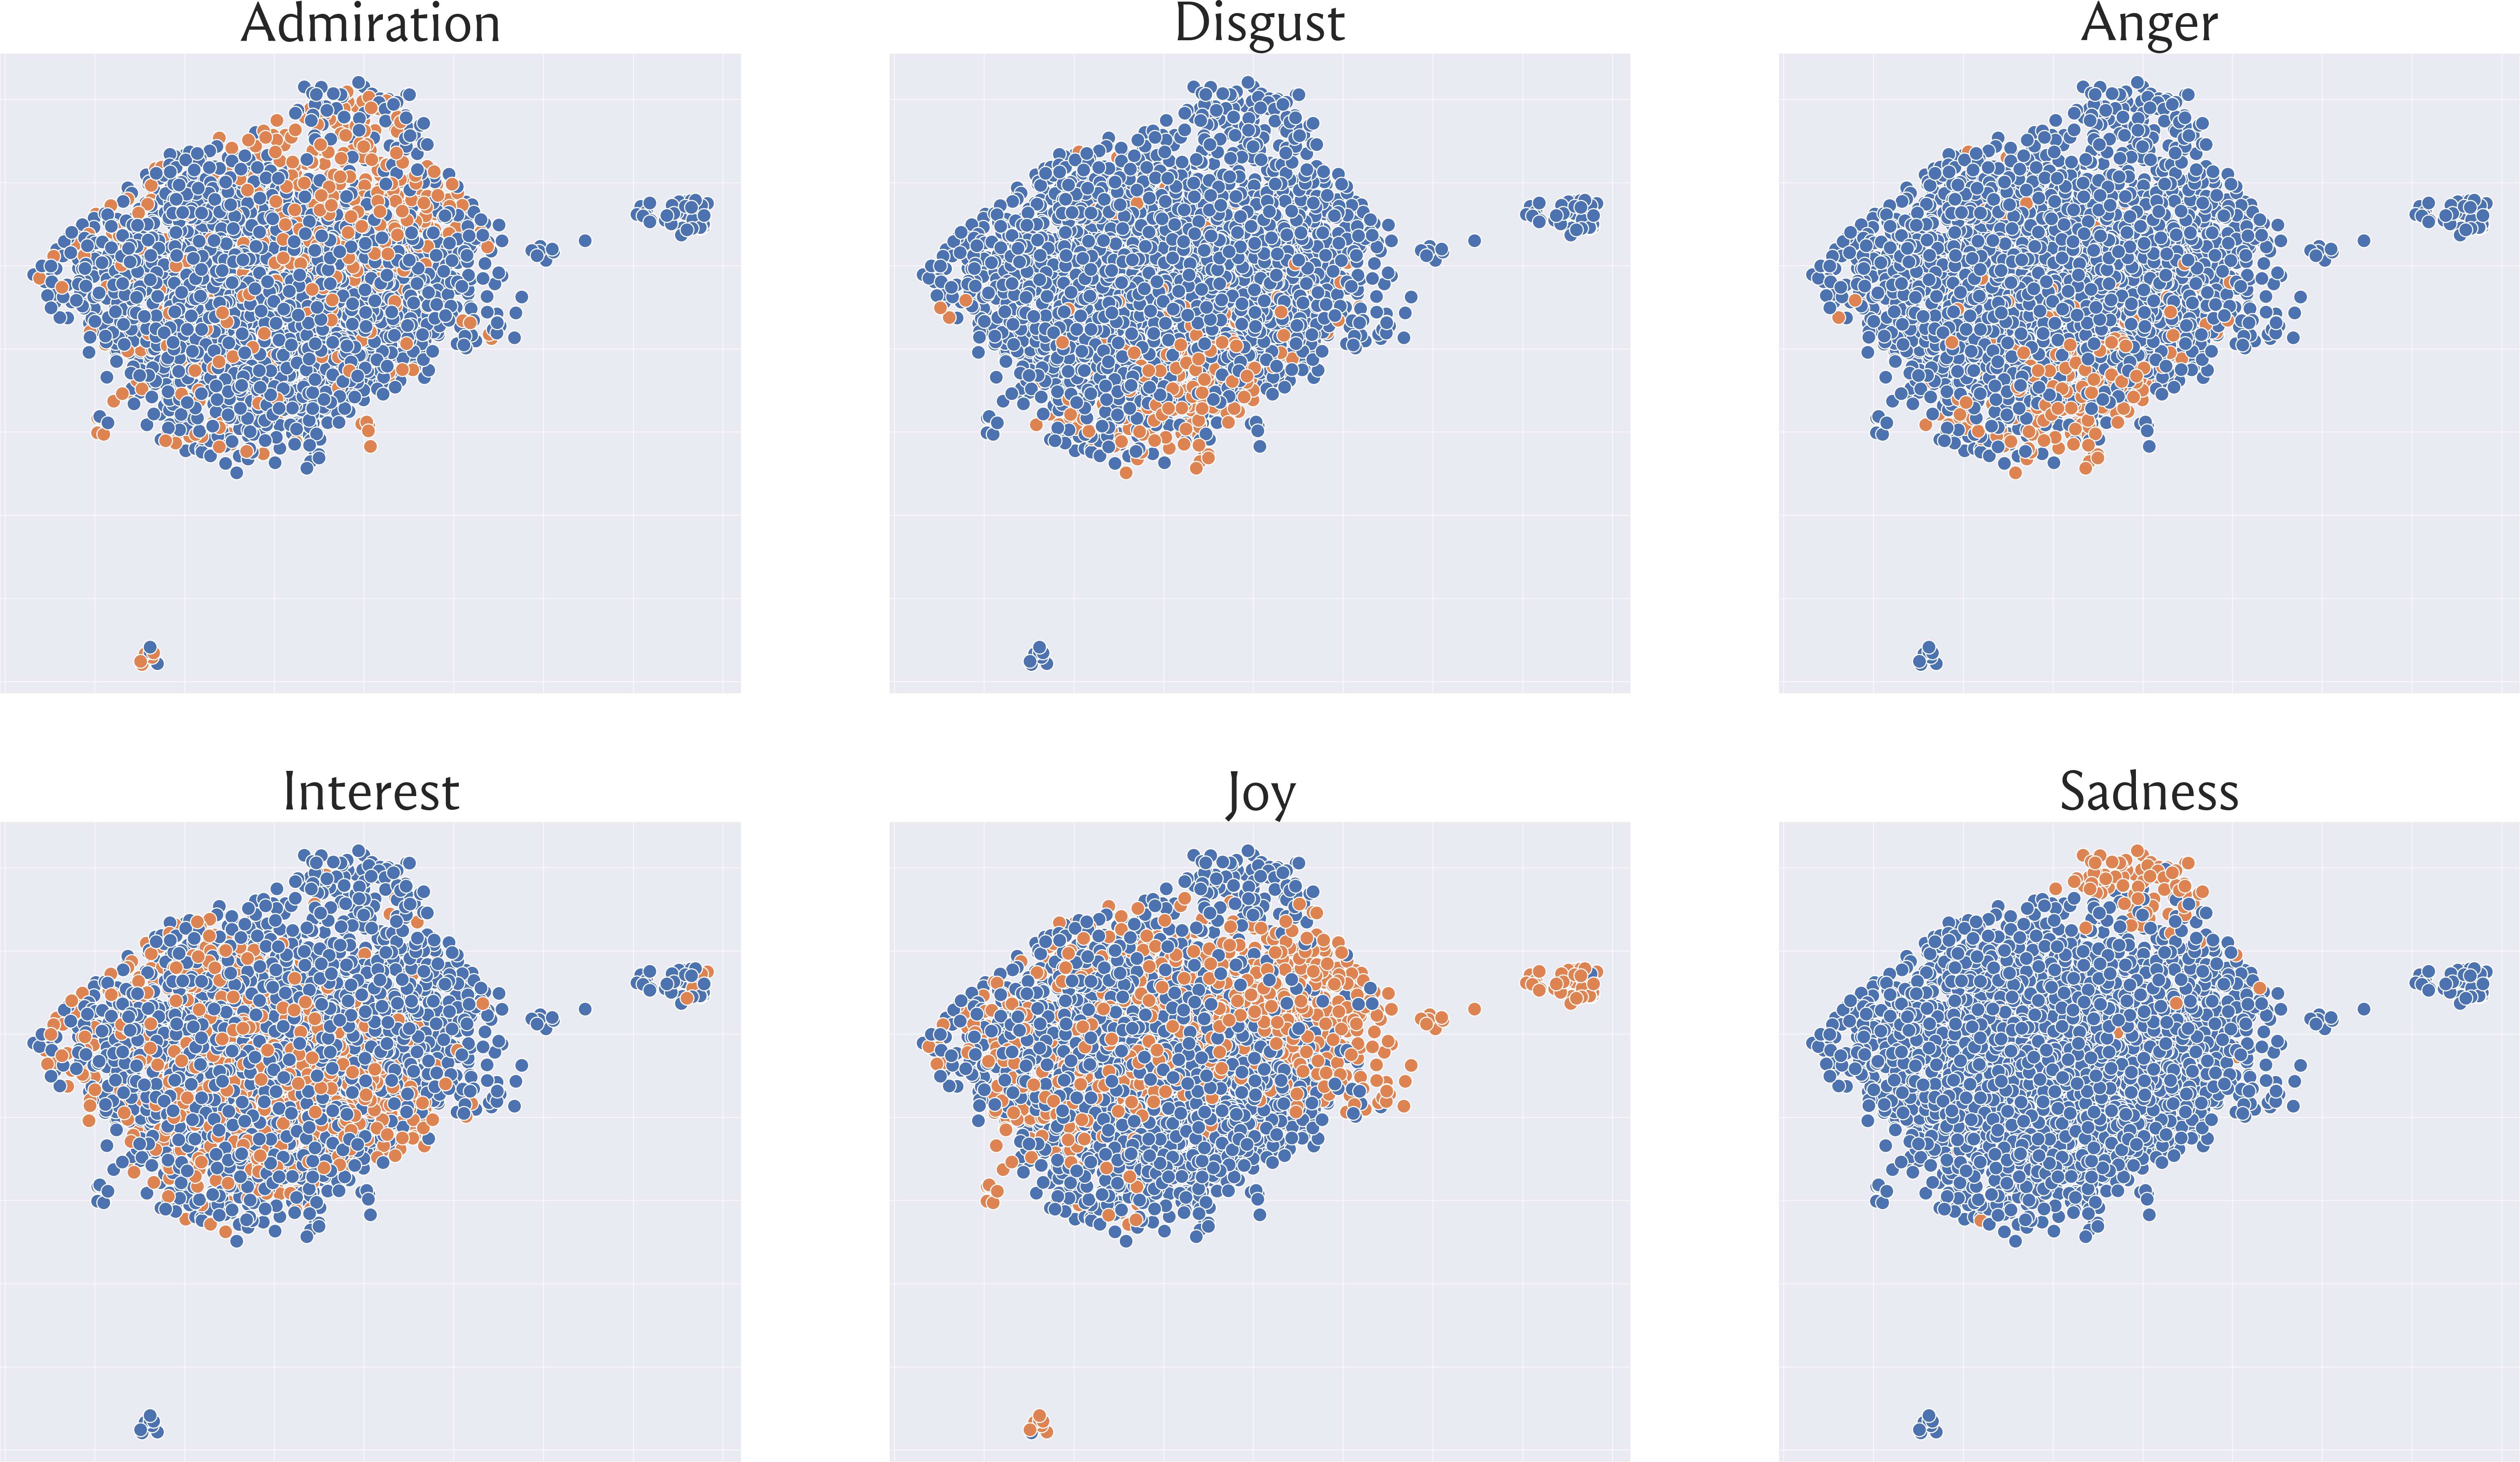
\includegraphics[width=\linewidth]{figures/bt_emots.png}
    \caption{Distribution of interpersonal emotions in unsupervised representations of tweets in our dataset. Orange indicates the emotion was present for that tweet. Each point represents one tweet from our dataset.}
    \label{fig:domainclus}
\end{figure*}

\paragraph{Can humans predict in/out-group?}

While our data naturally comes with ``gold'' IGR labels, what is unexplored is whether the distinction between in-group and out-group speech is prominent and noticeable by humans. Additionally, it is also unclear if humans might have their own expectation of how in/out-group speech should be characterized.

Concretely, we investigate if human annotators were capable of accurately performing the IGR prediction task when the speaker and target are masked. Two collaborators, one a social science graduate student, and the other a computational linguistics graduate student, annotated 50 random tweets from our validation data which they had not been exposed to earlier for in/out group labels. Their Fleiss $\kappa$ agreement score was 0.64, indicating moderate agreement.

To check how accurate their judgements were, we calculate for each annotator their F1 score against our ``gold'' in/out group labels. Their F1 scores on these 50 tweets were 0.67 and 0.63, which as we will discuss in Section~\ref{subsec:twitter-results}, only match simple baselines of supervised systems. Annotators comments indicate that they overly relied on the sentiment of tweets to make the classification --- positive sentiment means in-group and negative sentiment means out-group. While negative emotions are over-represented in out-group situations as Table~\ref{tab:inoutdist} shows, our dataset contains a substantial presence of out-group tweets with positive interpersonal emotions as well. Annotators also noticed some lexical cues like `bipartisan' that are indicative of out-group tweets.


\paragraph{Pre-trained representations capture interpersonal emotions} Pre-trained language models have been found to learn sentence representations that cluster by domain without supervision~\citep{aharoni-goldberg-2020-unsupervised}. We wished to investigate if any of our annotated properties cluster inherently in reduced representations of the tweets in our data. We use unsupervised representations from BERTweet~\citep{nguyen_bertweet_2020}, a language model pre-trained on 850M English tweets. We take the 768 dimensional embeddings from the final layer of the \texttt{<s>} token in BERTweet, and dimensionally reduce them to 2 dimensions using UMAP~\citep{sainburg2021parametric}. Figure~\ref{fig:domainclus} shows the distribution of tweets, color coded for interpersonal emotions. While there is a lot of overlap between representations when stratified by emotion, we can see that some emotions that are intuitively opposite, like admiration \& disgust, joy \& sadness are moderately separable. This indicates that interpersonal emotions do define some topic or domain level properties of a tweet.

\section{Modeling the intergroup bias}
\label{sec:twitter-model}

\subsection{Experiments}

We detail our experiments for the two novel tasks discussed in Section~\ref{sec:twitter-dimensions}: predicting the IGR (in-group or out-group) given a tweet, and predicting the interpersonal emotion given a tweet. We present baselines for the two tasks separately, and also present a multi-task model to gauge the extent to which knowledge of IGR may help in predicting interpersonal emotion, and vice versa.

\subsubsection{Intergroup Relationship}

\paragraph{Sentiment-Rule} Our first baseline is a rule-based one leveraging coarse sentiment: if a tweet's sentiment is predicted to be negative, classify it as out-group; if positive, classify it as in-group; and if neutral, classify it as either in-group or out-group randomly. We use a RoBERTa-Base model fine-tuned for sentiment on tweets~\citep{barbieri-etal-2020-tweeteval} to extract the sentiment of each tweet in our dataset.
    
\paragraph{NB-SVM} As a second baseline, we build an SVM model that uses Naive-Bayes log-counts ratios of unigrams and bigrams~\citep{wang-manning-2012-baselines}.


\paragraph{BERTweet} We use BERTweet~\citep{nguyen_bertweet_2020}, a language model pre-trained on 850M English tweets as our dataset consists purely of English language tweets. A classification head is placed on top of the language model. We also experiment with a version where the language model parameters are frozen, and only the classification head parameters are fine-tuned (BERTweet-ft).

The input to all models is only the tweet with no other context, and the target masked with a placeholder \texttt{@USER}.

\subsubsection{Interpersonal Emotion}

\paragraph{EmoLex} As a baseline model for interpersonal emotion identification, we rely on EmoLex~\citep{Mohammad2013CROWDSOURCINGAW}. EmoLex consists of 14,182 crowdsourced words associated with the 8 basic Plutchik emotions. Critically, these words appear in emotional contexts, but are not necessarily emotion words themselves. EmoLex counts occurrences of words from its lexicon in an utterance, and assigns a normalized score for each emotion based on occurrence frequency. We consider an emotion to be on, if it's normalized score is $\geq$ 0.001. While EmoLex has issues with regards to its context insensitivity and the social biases built into its lexicon~\citep{zad-etal-2021-hell}, we include it as a baseline to understand to what extent interpersonal emotions can be deduced using a lexicon.


\paragraph{BERTweet} We use the same BERTweet model as earlier. We add a dense output layer on top of the pretrained model for the purposes of finetuning, with a sigmoid cross entropy loss function to support multi-label classification. The loss is weighted for each of the 8 emotion labels with the ratio of positive and negative examples to increase precision. If none of the 8 emotion labels are flipped on, we consider that to be the `No Emotion' label, i.e. there is no interpersonal emotion between speaker and target in the tweet. We experiment with a version of the model where the language model parameters are frozen and only the labelling head parameters are fine-tuned (BERTweet-ft).

\subsubsection{Multi-Task Model}

In \textsection~\ref{sec:twitter-prelim}, we observed that the emotions anger and disgust are overwhelmingly present in out-group situations. Thus, we hypothesize that IGR information would be useful towards interpersonal emotion identification, and vice versa. To test this hypothesis we train a multi-task model. The model is trained to predict \emph{both} the IGR label and emotion using shared parameter finetuning.

We use the same BERTweet model as earlier. We add two dense output layers on top of the pretrained model, one for classifying IGR and another for labelling interpersonal emotion. Both heads share the same parameters below. These are trained with same loss as earlier individual models. The model alternates between finetuning for group relationship and emotion over every training item.

\subsubsection{Implementation}
We use \texttt{bertweet-base} pretrained embeddings from Huggingface~\citep{wolf-etal-2020-transformers}. All models are fine-tuned for a maximum of 20 epochs with early stopping. Early-stopping patience for models trained on each task separately is 3. The patience for the multi-task model is set at 5 as the multi-tasking setup led to slower convergence. The learning rate for the classification heads was set at 5e-3 while the learning rate for the internal language model parameters was set at 2e-5. Dropout probabilities in classification heads was set at 0.1. The best performing model before early stopping on validation data was chosen in all cases. We report F1 scores averaged over 3 random restarts for all models, with the standard deviation in parentheses next to the mean.

\subsection{Results and Analyses}
\label{subsec:twitter-results}

\begin{table}[t]
	\centering
	\begin{tabular}{lr|lr}
		\toprule
		\textbf{Model} & \textbf{F1} & \textbf{Model} & \textbf{F1} \\ \midrule
		Majority class & 51.1 & BERTweet & 74.1 (3.3) \\
		Sentiment-Rule & 56.3 & BERTweet-ft & 66.5 (1.6) \\
		NB-SVM & 62.5 & Multitask & 77.3 (0.8) \\
        Human & 66.7 & & \\
        \bottomrule
	\end{tabular}
	\caption{Results on test set, with SD in parentheses, for intergroup relationship prediction task.}
	\label{tab:inoutresults}
\end{table}


\paragraph{Intergroup relationship} In modeling IGR, we find that \texttt{Sentiment-Rule} performs not much better than chance (Table~\ref{tab:inoutresults}). This underscores one strength of our data, which contains a sizable number of out-group tweets with positive interpersonal emotion attached to them. The \texttt{NB-SVM} model based on unigrams and bigrams performs slightly better, and picks up on some obvious out-group lexical cues like the lemma `bipartisan', as shown in Table~\ref{tab:svm-features}. The \texttt{BERTweet} model performs substantially better, performing over 10 points better than humans. The model, with only the classification head fine-tuned, leaving the language model parameters intact(\texttt{BERTweet-ft}) performs about 10 points above chance --- indicating that there may be features advantageous towards this task in the vanilla LM itself.

\paragraph{Interpersonal Emotion}

We find that the \texttt{EmoLex} baseline, which relies purely on lexical cues, performs dismally on our data, with poor performance in both in-group and out-group settings(Table~\ref{tab:emoresults}). This is a strong indication that emotions are expressed more implicitly in this dataset. The \texttt{BERTweet} model performs substantially better, indicating that interpersonal emotions, even if implicit, can be learned.

\paragraph{Multitask Model}

As Table~\ref{tab:inoutresults} shows, Multi-tasking the two tasks leads to a noticeable improvement in F1 for IGR prediction, with the differences being statistically significant using a bootstrap test~\cite[p$<$0.05;][]{berg-kirkpatrick-etal-2012-empirical}; the multi-task model is also more stable with much lower variance across runs. These results suggest that interpersonal emotion is useful towards IGR prediction.

Table~\ref{tab:emoresults} shows that the performance of the multitask model on predicting interpersonal emotions is significantly better that the BERTweet model (p$<$0.05) on emotions like \emph{disgust}, which suggests that IGR is useful towards the task of emotion identification. Furthermore, multitasking boosted performance at predicting the \emph{no emotion} label by 20\%.  Table~\ref{tab:detemoresults} compares the multitask model's performance against the BERTweet model in \emph{out-group} settings (where most of the gains were found) for 3 emotions --- illustrating the boost in performance afforded by joint modeling of IGR and emotion for \emph{digust}. The 3 emotions listed also showed significant differences in their distribution in in-group and out-group settings.

\begin{table}[t]
    \centering
    \begin{tabular}{ll}
        \toprule
        \textbf{In-group} & \textbf{Out-group} \\ \midrule
        thanks, love, count me & thanks, bipartisan, restore \\
        birthday, my colleague & kind, resignation \\\bottomrule
    \end{tabular}
    \caption{Top unigram and bigram features from NB-SVM model for each class.}
    \label{tab:svm-features}
\end{table}


\paragraph{Humans vs.\ Models}

Comparatively, we find that model performance exceeds human performance on the task of in-group versus out-group prediction, albeit not on the same dataset. The model's main driver of performance is its high accuracy on positive intergroup emotion out-group tweets, such as those expressing admiration or joy. Human annotators consistently fall back on the heuristic that sentences with positive affect probably imply that the speaker is talking about someone in their in-group. But it is not the case in the political domain, where overtures to bipartisanship serve as useful signals. For instance, both \ref{ex:adm-1} and \ref{ex:adm-2} express admiration towards the target Doe, where the first is in-group while the second is out-group. The call to civility is the only subtle linguistic cue that this tweet may constitute out-group speech.

\ex. \a.\label{ex:adm-1} Admire @OfficialCBC Chairman @Doe's moral voice on issues of racism and restorative justice. He is a real leader for our nation and Congress.
     \b.\label{ex:adm-2} A decade has passed, but our friendship is the same. Proud to work with @Doe to \#ReviveCivility. \#tbt Read more about our efforts here:
     
Future work needs to look into what information the embeddings are using to make their classification decision.

\begin{table}[t]
	\centering
	\begin{tabular}{lrrrr}
		\toprule
		\textbf{} & \textbf{EmoLex} & \textbf{BERTweet} & \textbf{BERTweet-ft} & \textbf{Multi-task} \\\midrule
		Admir. & 37.5 & 70.3 (3.7) & 40.7 (1.1) & 68.9 (1.6) \\
		Anger & 26.6 & 71.3 (11.2) & 23.0 (3.4) & 69.3 (3.3) \\
		Disgust & 25.5 & 47.1 (21.6) & 13.0 (4.1) & 74.5 (7.1) \\
		Interest & 0 & 53.1 (3.3) & 5.8 (2.4) & 51.5 (8.5) \\
		Joy & 48.4 & 85.9 (1.9) & 71.3 (1.4) & 83.6 (1.3) \\
		Sadness & 4.3 & 11.1 (9.6) & 0 & 33.6 (18.5)\\
		\emph{No Emotion} & 22.2 & 49.1 (1.2) & 43.4 (3.8) & 71.6(1.2) \\\bottomrule
	\end{tabular}
	\caption{F1 scores on test set, with SD in parentheses, for interpersonal emotion labelling task.}
	\label{tab:emoresults}
\end{table}


\paragraph{Model Errors} While the multitasking setup improves model performance on the task of predicting IGR, and outperforms human labelers in our small pilot, it still gets some easy examples wrong, such as labelling~\ref{ex:disgust} as in-group even though it expresses some disgust at the target. The model also falls into the same trap as human labelers --- for instance assuming that a tweet expressing admiration must be in-group~\ref{ex:admiration}.

\ex.\label{ex:disgust} Trump selected @USER for HHS Secretary. Price has undeniable history of cutting access to healthcare to millions, especially women.

\ex. \label{ex:admiration} Inspiring speech from @USER - we have a duty to represent our country with respect \& dignity. \#NationalDayofCivility.

To ensure that model performance on IGR prediction is not limited by the size of our training data, we experimented with training \texttt{BERTweet} models on larger datasets. Since we have `found supervision' for IGR labels, we only need to increase training data size by sampling more tweets from relevant accounts using the same procedure detailed in \textsection~\ref{subsec:twitter-datasources}. We found that F1 score does not increase with more training data.

Future work needs to look into linguistically motivated ways to improve model performance on the IGR task. Since we have observed that the multi-task setup improves model performance, perhaps other multi-task setups, such as modeling the overall affect towards the target expressed by the speaker might help in modeling IGR better.

\begin{table}[t]
	\centering
	\begin{tabular}{lrr}
		\toprule
		\textbf{Emotion} & \textbf{BERTweet} & \textbf{MultiTask} \\\midrule
		Admiration & 77.9 (2.6) & 72.8 (3.9)\\
        Anger & 71.7 (9.9) & 69.4 (3.4)\\
        Disgust & 48.2 (22.4) & 75.9 (6.5)*\\\bottomrule
	\end{tabular}
	\caption{F1 scores on test set, SD in parentheses on out-group tweets. * indicates statistical significance (p<0.05)}
	\label{tab:detemoresults}
\end{table}


\section{Discussion \& Conclusion}

Taking a cue from studies of bias in social science and psychology, we situate bias in language use through the lens of interpersonal relationships between the speaker and target of an utterance, and the speaker's interpersonal emotional state with respect to the target. Over a corpus of tweets by members of US Congress,  we introduce two novel tasks -- intergroup relationship prediction (IGR) and interpersonal emotion labelling, to better understand variation in language as a function of social relationship between speaker and target in interpersonal utterances. We find certain interpersonal emotions like anger and disgust are over-represented in out-group situations, with the majority of the negative emotions directed at leaders of the two political parties. Through modeling studies, we find that transformer based models perform better than humans at predicting IGR given an utterance, raising the question as to what latent features of language the model uses to make this decision. Finally, we also find that joint modeling of the two dimensions is beneficial to prediction of certain interpersonal emotions in out-group situations. 


This chapter lays the groundwork for future studies into intergroup bias more broadly. Analysis and modeling prove that intergroup bias can be systematically studied by decomposing it into discrete dimensions, and subtle variations can be captured using pre-trained language models fine-tuned for our task. Building upon the dataset and results in this chapter, we circle back to our motivations --- \textbf{what are the systematic linguistic variations between in-group and out-group speech?}. The next chapter attempts to answer this question, through focused probing experiments into the neural models trained to discriminate in-group tweets from out-group tweets; Probing seeks to understand if the neural models learns to use human-interpretable higher-order linguistic features when performing the task.



\chapter{Intergroup bias gets a counterfactual probe}
\label{chapter:probing}

In the last chapter, we proposed a new framing of bias by modeling intergroup relationships (IGR, in-group and out-group) in interpersonal English language tweets, potentially capturing more subtle forms of bias. Analyses showed that this was a worthwhile framing of bias to understand it more comprehensively, but it raises a new question: which \emph{linguistic features} vary systematically in different intergroup contexts?

As described in Chapter~\ref{chapter:intro}, LIB speculates that socially desirable in-group behaviors and socially undesirable out-group behaviors are encoded at a higher level of \textbf{abstraction}. The theory however relies on a restricted definition of abstractness that relies solely on predicates, and an ad-hoc analysis of `social desirability' that doesn't permit large-scale analysis. We can do better by using two well-defined pragmatic features: \emph{specificity}~\citep{li_discourse_2017} is a pragmatic feature of text that measures the level of detail (similar to abstract--concrete axis), while \emph{affect} is a feature that measures the attitude of a speaker towards their target~\citep{sheng-etal-2019-woman} in an utterance (analogous to social desirability).

Specificity and affect are analogous to the LIB axes of language variation that are easy to annotate and compute. Furthermore, specificity is a more \emph{general} property than abstractness in the LIB --- specificity is a property of the whole sentence rather than just the predicate. Thus, our study focuses intergroup bias more generally, rather than the narrow parameterization of the LIB. Similar to the LIB, our formulation of intergroup bias predicts that positive affect in-group utterances and negative affect out-group utterances are encoded with \emph{lower specificity} (i.e. more generally). Tables~\ref{tab:lib} and \ref{tab:ib} compare the predicted language variation between the LIB and our formulation. 

In this work, we perform the first large-scale study of linguistic differences in intergroup bias by analyzing its nature in the corpus of English tweets described in \textsection~\ref{subsec:twitter-datasources}, which makes use of naturally occurring labels for in-group vs. out-group. This distinguishes us from existing work in LIB which mostly relies on artificial responses from participants in studies, rather than natural language use in the wild. To bolster our probing investigation, we also explore it causally: exploiting the quantitative nature of our formulation to study if a neural model fine-tuned for IGR prediction uses pragmatic features such as specificity and affect in its decision-making process through counterfactual probing techniques~\citep{ravfogel-etal-2021-counterfactual}.

To summarize our findings, we find a modest positive correlation between affect and IGR in our data, with a positive causation effect as well --- making a tweet's affect more positive makes it more likely to be in-group regardless of its specificity. We find no correlation between specificity and IGR in our data. Surprisingly, we discover a causal effect of low specificity on IGR prediction that is uniform across affect, but none for high specificity. We hypothesize that this could be because of damage to the underlying language model, but we leave further investigation to future work. We release our code and data \href{https://github.com/venkatasg/intergroup-probing}{online}.

\section{Prior Work}

\paragraph{Intergroup bias} The  Linguistic Intergroup Bias  (LIB) theory~\cite{maass_language_1989,maass_linguistic_1999} tries to explain how stereotypes are transmitted and persist in communication by hypothesizing that socially desirable in-group behaviors and socially undesirable out-group behaviors are encoded at a higher level of abstraction . The LIB has been reproduced in various psychological experiments and analyses~\cite{Anolli2006LinguisticIB, gorham_news_2006}; it has also been used as an indicator for a speaker’s prejudicial attitudes~\cite{hippel_linguistic_1997}, and racism~\cite{schnake_modern_1998}. 

Table~\ref{tab:lib} describes the LIB asymmetry and the parameters used. As stated earlier, the LIB relies on ad-hoc and hand-coded concepts such as `social desirability' and abstractness of predicates~\citep{semin_cognitive_1988} . Our proposed experiments \emph{generalize} beyond the LIB by utilizing parameters that are easily computable, and are a function of the whole utterance.

\paragraph{Specificity} Specificity is a pragmatic concept of text that measures the level of detail and involvement of concepts, objects and events. \citet{louis-nenkova-2011-text} introduced the first dataset and model for sentence specificity prediction, and in later work \citet{li_discourse_2017} illustrated the role of specificity in discourse coherence. Furthermore, \citet{gao_predicting_2019} expanded the scope of specificity analysis from the news domain to social media.

\begin{table}[t]
    \centering
    \begin{tabular}{lll}
     \toprule
        \textbf{} & \textbf{in-group} & \textbf{out-group} \\ \midrule
        positive affect & low specificity &  high specificity \\ \midrule
        negative affect & high specificity & low specificity \\ 
    \bottomrule
    \end{tabular}
    \caption{Predicted language variation in our more general formulation, using specificity and affect}
    \label{tab:ib}
\end{table}


\paragraph{Affect} There is a wealth of work studying emotions and sentiment in social media text~\citep{mohammad-2012-emotional,6406313, Mohammad2015UsingHT, abdul-mageed-ungar-2017-emonet,desai-etal-2020-detecting,demszky-etal-2020-goemotions}. We introduced the first dataset annotated for \emph{interpersonal} emotion (defined as only emotions expressed towards or in connection with a target), using the Plutchik wheel~\citep{plutchik2001nature} as a framework. While fine-grained, this approach isn't amenable to the experimentation we propose easily. Inspired by the concept of \emph{regard} by a speaker towards a demographic in an utterance~\citep{sheng-etal-2019-woman}, we introduce annotations for a coarse-grained feature we term \emph{affect} that estimates how a speaker feels towards the target they mentioned in an interpersonal utterance.

Table~\ref{tab:ib} describes the intergroup language variation as hypothesized in our experimentation, using specificity and affect. Analogous to LIB, our hypothesis is that positive affect utterances directed at in-group individuals, and negative affect utterances directed at out-group individuals are encoded with \emph{lower specificity}.

\paragraph{AlterRep} AlterRep~\citep{ravfogel-etal-2021-counterfactual} is a probing technique that tests if a neural network \emph{uses} a property, rather than just testing if the model's learned representations correlate with the property. The method uses Iterative Nullspace Projection~\citep[INLP;][]{ravfogel-etal-2020-null} to iteratively train a linear classifier on the model's internal representations to pick out a particular feature, using the parameters learned by the classifier to intervene on the embedding and alter it in a systematic way. The AlterRep method based on INLP has been used to probe for syntactic phenomena such as subject-verb number agreement~\citep{ravfogel-etal-2021-counterfactual}. To our knowledge, ours is the first work probing if a model learns and uses higher-level pragmatic features like affect and specificity using AlterRep.

\section{Probing for the intergroup bias}

\subsection{Data \& Annotations}
\label{subsec:data}

We use the same dataset of tweets from \textsection~\ref{subsec:twitter-datasources}, which consists of tweets by members of US Congress that @-mention other members in the same tweet, with `found-supervision' for the IGR labels of every tweet. A tweet is in-group if it is targeted at another member of the same party as the writer of the tweet, else it is out-group.

\paragraph{Affect}
We build upon the dataset's fine-grained annotations for interpersonal emotion by adding annotations for affect. We presented annotators on Mechanical Turk with tweets from our dataset with the target mention masked (with the placeholder \@Doe, to minimize potential biases of the annotator), and asked the following questions:

\begin{enumerate}
    \item[a.] How does the writer feel in general about \@Doe? \emph{warmly, coldly, neutral, mixed}
    \item[b.] How does the writer feel in general about \@Doe's actions/behavior? \emph{approval, disapproval, neutral, mixed}
\end{enumerate}

Annotators are given the option to select one of the 4 options listed above for each question. For each tweet, we collect annotations from 3 annotators, obtaining an aggregate label for each question by majority vote. We report an inter-annotator agreement score ~\citep[Fleiss's kappa;][]{fleiss1971measuring} of 0.53 for the first question, and 0.56 for the second.

We derive a binary affect label ($\pm 1$) from our annotations using a simple rule: If the writer of a tweet is deemed to either feel warmly towards the target, or if they approve of the target's actions, the affect is set to be positive; else it is set to be negative. An analysis of our collected annotations on the data shows that there is a small positive (Pearson's) correlation ($r$=$0.2$, $p<0.001$) between binary affect and IGR.


\paragraph{Specificity} Specificity of the tweets in the dataset are calculated using the specificity  prediction tool from \citet{gao_predicting_2019}. Their specificity predictor is trained on tweets, and uses surface lexical features, as well as syntactic, semantic and distributional features to calculate a specificity score between 1 and 5. We note that on our dataset, there was \emph{no correlation between specificity and IGR} ($r$=$-0.07$, $p<0.001$), unlike affect. On further inspection of our dataset, we find that tweets with very high/low specificity scores \citep[gathered by excluding specificity scores between 3 and 4, similar to excluding the middle in][]{gelman2009} have a small but statistically significant negative correlation with IGR labels ($r$=$-0.13$, $p<0.001$).

\subsection{Data \& Annotation}
\label{subsec:probing-data}

\begin{table}[t]
	\centering
	\begin{tabular}{lrrr}
		\toprule
		\textbf{Affect} & \textbf{Train} & \textbf{Dev} & \textbf{Test} \\ \midrule
		Positive & 1813 & 226 & 242\\
        Negative & 589 & 80 & 83\\
        \bottomrule
	\end{tabular}
	\caption{Distribution of affect in train-dev-test split}
	\label{tab:affect-traindevtestsplit}
\end{table}


To obtain reliable annotations, we prequalify annotators using a qualifying task. Annotators were recruited on Mechanical Turk using a qualifying task where they were asked to annotate 6 tweets using the schema detailed in\textsection~\ref{subsec:data}. We restricted the qualification task to annotators living in the USA who had attempted at least 500 HITS and had a HIT approval rate $\geq$ 98\%. After manual inspection, 6 anonymous annotators were qualified for bulk annotation. Each tweet was annotated by three different annotators. To ensure annotators were paid a fair wage of at least 10\$ an hour, we paid annotators \$0.50 per HIT. Each HIT involved annotating 3 tweets, which we estimate to take on average 3 minutes to complete.  In total, 3,033 tweets between 2010 and 2021 were annotated with perceived affect.

We present preliminary statistics for the annotations on the dataset of tweets in Table~\ref{tab:traindevtestsplit}.

\subsection{Interventions}
\label{subsec:interventions}

\begin{figure}[t]
    \centering
    \begin{tikzpicture}
	\begin{axis}[
		xlabel={INLP iterations},
		% ylabel={LM Top-100 accuracy},
        axis x line*=bottom,
        y axis line style= { draw opacity=0 },
        ymajorgrids=true,
        xtick={8,16,24,32,40,48,56,64},
        enlarge x limits=-1,
        ymin=0,
        ymax=100,
        legend columns=2,
        height=0.4\textheight,
        width=\linewidth,
        legend style={at={(0.5,1.2)},anchor=north, draw=none},
          legend entries={Push positive affect,
                          Push negative affect,
                          Push specific,
                          Push general
                          }
    ]
    \addplot[only marks, color=TolTeal, mark=*, mark size=2pt] table [x=inlp, y=posaff, col sep=tab] {data/lmacc.tsv};

    \addplot[only marks, color=TolWine, mark=*,, mark size=2pt] table [x=inlp, y=negaff, col sep=tab] {data/lmacc.tsv};

    \addplot[only marks, color=TolTeal, mark=triangle*, mark size=2pt] table [x=inlp, y=spec, col sep=tab] {data/lmacc.tsv};
    
    \addplot[only marks, color=TolWine, mark=triangle*, mark size=2pt] table [x=inlp, y=general, col sep=tab] {data/lmacc.tsv};
	\end{axis}
\end{tikzpicture}

    \caption{Top-100 LM Accuracy on train plus validation split of our dataset for different intervention strengths.}
    \label{fig:lm-acc}
\end{figure}

\paragraph{Model} We use BERTweet~\citep{nguyen_bertweet_2020}, a language model pre-trained on 850M English tweets, the same model used in \textsection~\ref{sec:twitter-model}. All intervention experiments are carried out with the best performing \emph{fine-tuned} version of this model --- where the model is fine-tuned on the task of predicting IGR labels. The input to the model is only the tweet with no other context, and the target masked with a placeholder \texttt{@USER}.

We use the model's representations from layer 11 for the INLP procedure since it shows the most reliable effects. INLP \citep{ravfogel-etal-2020-null} works by learning a series of linear classifiers on the representations from an encoder. In each iteration, the embeddings are projected onto the intersection of nullspaces of the classifiers learned so far, meaning the information used by the existing classifiers is removed from the model. Every subsequent classifier we learn removes more information of the property of interest from the model's representations.  We find that higher layers offer a good balance between feature extractability and language model stability (see Figure~\ref{fig:lm-acc}) for our features. 

After training INLP, AlterRep uses the classifier's decision space to project model embeddings into a null component that contains no information from the feature of interest, and an orthogonal component, that contains all the information from the feature of interest. These two components thus enable us to perform the counterfactual intervention --- pushing model embeddings towards having more, or less, of a particular property. When AlterRep uses INLP classifiers with more iterations, the strength of the intervention is greater. Figure~\ref{fig:flowchart} offers an illustration of our intervention experiment on specificity, and the expected results.

\paragraph{Affect} Using the binary affect labels we derived from annotations that we described in \textsection~\ref{subsec:data}, we perform interventions to test if the model uses affect causally in its decision. We sample 3 tokens at random from each sentence in the training and validation split of our dataset, train an iterative linear classifier on the model's representations of these tokens using INLP (against the affect label of the tweet), and use the decision boundary learned by the classifier to intervene by pushing model representations to have more positive affect or have more negative affect. We set the hyperparameter $\alpha$ in AlterRep to 4.


\paragraph{Specificity} The INLP classifier for specificity is learned using the same procedure as for affect. We train the classifier on only the tweets with high and low specificity scores in our dataset (scores below 3 and above 4; scores taken from the specificity prediction tool in \citet{gao_predicting_2019}), excluding the middle to ensure effective learning of the decision boundary~\citep{gelman2009}. Thus, we are effectively pushing the model representations to have high or low specificity. For both affect and specificity, once the INLP classifier is learned, we perform the intervention on a random subset of 30\% of the tokens of a tweet (to control for tweet length). We also report the results of random interventions as a control, where random interventions are generated by sampling from a standard gaussian instead of using the decision matrix generated by INLP.

\begin{figure*}[t]
    \centering
    \begin{tikzpicture}[node distance = 0.1\textwidth, auto]
    % Place nodes
    \node (middle-plot) {
        \begin{tikzpicture}
            \begin{axis}[ybar, ymin=0,ymax=100,
                         symbolic x coords={+ve,-ve},xtick=data,  /pgf/bar width=2em, width=0.25\textwidth,height=0.2\textheight, tick label style={font=\small}, yticklabels=None, enlarge x limits=0.35, ytick style={draw=none}, xlabel={\small Affect}, ylabel={\small\% in-group}]
                \addplot+[ybar, color=TolIndigo!50]
                    coordinates {(+ve,40) (-ve,60)};
            \end{axis}
        \end{tikzpicture}
    };
    \node [left of=middle-plot, xshift=-0.2\textwidth] (left-plot) {
        \begin{tikzpicture}
            \begin{axis}[ybar, ymin=0,ymax=100, ylabel={Hate Speech \%},
                         symbolic x coords={+ve,-ve},xtick=data,  /pgf/bar width=2em, width=0.25\textwidth,height=0.2\textheight, tick label style={font=\small},yticklabels=None, enlarge x limits=0.35, ytick style={draw=none}, xlabel={\small Affect}, ylabel={\small\% in-group}]
                \addplot+[ybar, color=TolIndigo!50]
                    coordinates {(+ve,20) (-ve,90)};
            \end{axis}
        \end{tikzpicture}
    };
    \node [right of=middle-plot, xshift=0.2\textwidth] (right-plot) {
        \begin{tikzpicture}
            \begin{axis}[ybar, ymin=0,ymax=100,
                         symbolic x coords={+ve,-ve},xtick=data, /pgf/bar width=2em, width=0.25\textwidth,height=0.2\textheight, tick label style={font=\small},yticklabels=None, enlarge x limits=0.35, ytick style={draw=none}, xlabel={\small Affect}, ylabel={\small\% in-group}]
                \addplot+[ybar, color=TolIndigo!50]
                    coordinates {(+ve,90) (-ve,10)};
            \end{axis}
        \end{tikzpicture}
    };
    \node [block, below of=middle-plot, yshift=-0.1\textheight] (bert-1) {\small $h_i$};
    \node [block, left of=bert-1, xshift=-0.2\textwidth] (bert-pos) {\small $h_i^s$};
    \node [block, right of=bert-1, xshift=0.2\textwidth] (bert-neg) {\small $h_i^g$};
    
    \node [block, below of=bert-1, yshift=-0.1\textheight] (bert) {\small  $h_i$};
    \node [cloud, below of=bert-pos, yshift=-0.1\textheight] (pos) {\shortstack{\small  push token embeddings\\\small  towards high specificity}};
    \node [cloud, below of=bert-neg, yshift=-0.1\textheight] (neg) {\shortstack{\small  push token embeddings\\\small  towards low specificity}};
    
    \node [tweet, below of=bert, yshift=-0.05\textheight] (tweet) {\small Thanks, \@USER for joining me in demanding \#PaperBallotsNOW};
    
    % Draw edges
    \path [line] (tweet) -- node {\small  get embeddings with BERTweet}(bert);
    \path [line] (bert) -- (bert-1);
    \path [line] (pos) -- (bert-pos);
    \path [line] (neg) -- (bert-neg);
    \path [line] (bert) -- (pos);
    \path [line] (bert) -- (neg);
    \path [line] (bert-1) -- node[pos=0.5,left] {\small In or Out-Group?}(middle-plot);
    \path [line] (bert-neg) -- node[pos=0.5,left] {\small In or Out-Group?}(right-plot);
    \path [line] (bert-pos) -- node[pos=0.5,left] {\small In or Out-Group?}(left-plot);
    \draw[latex'-latex'] (left-plot) -- node {\tiny Compare}(middle-plot);
    \draw[latex'-latex'] (middle-plot) -- node {\tiny Compare}(right-plot);
\end{tikzpicture}

    \caption{Flowchart describing the specificity intervention experiment and expected results.}
    \label{fig:flowchart}
\end{figure*}

\paragraph{Hypotheses} We report the percentage of tweets in the test split of our dataset that are predicted to be in-group by our classifier model with increasing strength of the intervention (number of INLP iterations, 0 being pre-intervention). Thus, we have the following hypotheses on the effects of our intervention on the data based on our intergroup bias framework described in Table~\ref{tab:ib}:

\begin{enumerate}
    \item Interventions towards positive affect should induce the model to predict low specificity  tweets to be in-group and high specificity tweets to be out-group, while interventions towards negative affect should affect the model conversely.
    \item Interventions towards higher specificity should induce the model to predict positive affect tweets as out-group and negative affect tweets as in-group, while interventions towards lower specificity should affect the model conversely.
\end{enumerate}

\subsection{Results \& Analysis}

The results for the interventions on affect are presented in Figure~\ref{fig:affect}, while those for specificity are presented in Figure~\ref{fig:spec}. Overall, we observe that in both cases, interventions had the same effect on tweets that were annotated with positive affect as they did on tweets with negative affect (and similarly for tweets with high and low specificity) --- so we only show the percentage of \emph{all} tweets in the test split classified as in-group.

\paragraph{Affect} As Figure~\ref{fig:affect} shows, pushing model representations towards having more positive affect causes almost all tweets in the test split of our data to be classified as in-group after 32 iterations of INLP. The randomness after 40 iterations of INLP could be attributed to the underlying RoBERTa language model being destroyed, as the LM Top-100 accuracy plot in Figure~\ref{fig:lm-acc} shows. Pushing the model's representations towards negative affect shows the inverse effect as expected, although the nature of the drop appears different. We hypothesize that this is because most of the tweets in our dataset (75.2\%) have positive affect. An intervention pushing the representations towards negative affect would be slower and require stronger intervention forces, which is borne out in Figure~\ref{fig:affect}.

\begin{figure}[t]
    \centering
    \input{figures/affect.tex}
    \caption{\% of test set classified as in-group plotted against number of INLP interventions for affect.}
    \label{fig:affect}
\end{figure}

\paragraph{Specificity} Figure~\ref{fig:spec} shows that pushing model representations to be more specific has no effect on model behavior and is indistinguishable from the control; but pushing towards lower specificity has a noticeable effect --- interventions after 48 iterations of iNLP lead to all the data being predicted as in-group. Our hypothesis states that general language is more likely in positive affect in-group contexts; however we find no difference in the model's behavior on positive versus negative affect tweets as reported earlier.

Overall our findings indicate that while the model does use affect towards making its decision on the intergroup relationship prediction task (albeit uniformly across specificity), it doesn't use specificity as we had predicted. The discrepancy between high and low specificity interventions could be because the average specificity of tweets in our training data is 3.49 ($\sigma=0.54$) --- meaning that interventions towards lower specificity act in opposition to most of our data in representation space. But these results requires further investigation to understand them better.

\begin{figure}[t]
    \centering
    \begin{tikzpicture}
	\begin{axis}[
		xlabel={INLP iterations},
		% ylabel={F1 Score/\In-group},
        axis x line*=bottom,
        y axis line style= { draw opacity=0 },
        ymajorgrids=true,
        xtick={8,16,24,32,40,48,56,64},
        enlarge x limits=-1,
        ymin=0,
        ymax=100,
        height=0.4\textheight,
        width=\linewidth,
        legend columns=-1,
        legend style={font=\small, at={(0.5,1.2)},anchor=north, draw=none, /tikz/every even column/.append style={column sep=0.03\columnwidth}},
          legend entries={Push high specificity,
                          Push low specificity,
                          Controls
                          }
    ]
    \addplot[only marks, thick, color=TolTeal, mark=*, mark size=2pt] table [x=inlp, y=posspec, col sep=tab] {data/test.tsv};
    
    \addplot[only marks, thick, color=TolWine, mark=triangle*, mark size=2pt] table [x=inlp, y=negspec, col sep=tab] {data/test.tsv};
    
    \addplot[only marks, thick, color=black!60, mark=x, mark size=2pt] table [x=inlp, y=posspec-control, col sep=tab] {data/test.tsv};
    
    \addplot[only marks, thick, color=black!60, mark=x, mark size=2pt] table [x=inlp, y=negspec-control, col sep=tab] {data/test.tsv};
	\end{axis}
\end{tikzpicture}

    \caption{\% of test set classified as in-group plotted against number of INLP interventions for specificity.}
    \label{fig:spec}
\end{figure}

\paragraph{Qualitative error analysis} Digging into the results further, we wanted to investigate if the interventions function the way we wanted them to. We analyzed the tokens that the model predicts before and after intervention for example \ref{ex:qual}. Firstly, finetuning the model for IGR prediction leads to degradation in LM abilities --- a vanilla model predicts \emph{birthday, anniversary} for the masked token in \ref{ex:qual}, but the fine-tuned model predicts nonsensical tokens like \emph{sworn, opport\_\_} even before any interventions. Pushing towards negative affect causes it to predict tokens with negative connotations (\emph{killing, ass, opposition}), but degrades the underlying LM even further. The specificity interventions are especially hard to interpret due to the semantically and syntactically implausible tokens being selected (\emph{opport\_\_, mug\_\_, ask\_\_}) 

\ex.\label{ex:qual} Happy <mask> @USER! I got you a new bill: \#IIOA

While some of the interventions push the model's predictions to be in the general lexical space desired (which probably explain the affect intervention results), the lack of contextual fit due to LM degradation may explain the inconclusive results, and lack of interaction between affect and specificity.

\section{Discussion \& Conclusion}

In this chapter, we performed a correlational and causal analysis of two pragmatic features, specificity and affect, on a dataset of interpersonal tweets in English, to establish how they influence intergroup relationship prediction. We find modest correlations between our features and IGR labels, while counterfactual probing reveals mixed results. Affect influences IGR prediction causally but without interacting with specificity, while specificity only influences IGR prediction in one direction. 

Overall, we found no evidence for our general intergroup bias hypothesis, described in Table~\ref{tab:ib}. While disappointing, the findings in this chapter are still instructive towards our next steps. There are 2 major issues that need to be addressed, if we are to truly discover systematic linguistic variations that different in-group speech from out-group speech:

\begin{enumerate}
    \item We need diverse real-world data, that reflects natural language use, at a larger scale. While our dataset of political tweets has served us well, it is limited in terms of its utility. Many of the tweets themselves are composed by social media teams employed by politicians, and are composed with political gain in mind. Moreover, the volume of tweets, and the representative groups in the context of U.S politics are small. We also need ample, high-quality data to build reliable computational models for prediction and analysis of the intergroup bias.
    \item The data needs to be tied to real-world events. Currently, both axes of variation in our novel hypothesis, affect and specificity, are both features derived from the utterance. This confounds analysis and discovery of variation between groups --- the LIB describes asymmetrical linguistic changes in abstractness in response to variation in acceptability of real-world behaviors (social desirability). We attempted to approximate social desirability through affect, but we don't have access to the direct affect of the speaker towards a referent, and this is impossible to obtain at scale. Thus, we need a robust measurement of a variable that describes the \textbf{state-of-the-world} preceding an utterance.
\end{enumerate}

We tackle both of these issues directly in the next Chapter by introducing a novel dataset of online sports comments \emph{parallel} with sports games --- tying linguistic behavior to events directly. 


\chapter{Intergroup bias in Reddit NFL game comments}
\label{chapter:football}

\begin{center}
    \textit{\textellipsis a socially acceptable outlet for xenophobia. That is the function of organized sports (in society) for the most part\textellipsis}
    \\\hspace{4em}---John Siracusa, \href{https://www.relay.fm/rd/3}{Reconcilable Differences Ep. 3}
\end{center}

Chapter~\ref{chapter:twitter} described my first data-driven study of intergroup bias in real-world language use, by curating a dataset of tweets by members of U.S. Congress with metadata derived gold labels for intergroup relationship. Crowd-sourced annotation revealed the systematic variation of interpersonal emotion with intergroup labels, and modeling further reinforced the systematic interaction between these two variables. In the previous chapter, I described my probing experiment to discover if the interaction between specificity and affect could describe any of the systematic \emph{linguistic} variation observed in the data. While the results were inconclusive, they were instructive towards how we needed to proceed towards answering this question --- we needed to look within utterances for intergroup variations in how people \textbf{referred} to the in-group and out-group, and we needed to \emph{tie} the variation in intergroup language to the events preceding the utterance.

As I have described earlier, the LIB hypothesis is limiting and ad-hoc towards capturing the rich forms of variation that we do observe in natural language. For instance, the dataset of political tweets was restricted to tweets where there was only one explicit referent (via @-mentions). However, the \textbf{form of referencing} the in-group or out-group can reveal subtle biases as well. Consider these tweets:

\ex. \label{ex:trump-tweets} \a.\label{ex:trump-tweet-1} \textbf{Mr. President}- Please tell your supporters to STAND DOWN, LEAVE the Capitol grounds and obey law enforcement who once again are risking their lives for our country!\textellipsis
    \b. \label{ex:trump-tweet-2} \textellipsis~Americans deserve answers on these unacceptable delays. We need a full accounting of \textbf{Pres Trump} and defense officials’ decisions on Jan 6~\textellipsis
    \b. \label{ex:trump-tweet-3} We survived an insurrection and \textellipsis~In we made it clear what St. Louis already knew: \textbf{Donald Trump} was the white supremacist-in-chief.

All of these tweets \emph{refer} to the same individual --- Donald Trump. However, \ref{ex:trump-tweet-1} is by a Republican Congresswoman (and thus in-group), while \ref{ex:trump-tweet-2} and \ref{ex:trump-tweet-3} are by Democrats (out-group). One can observe distinct changes in how the speakers \emph{refer} to him that is tinged by their (intergroup) relationships and changes in state-of-the-world. The Republican's tweet is more respectful, by only referring to him by position rather than name.  The LIB hypothesizes variation only in the form of the predicate --- this is an acceptable simplification when eliciting experiments in utterances, but discards useful information, as illustrated in these examples, in real-world language use.

To decipher the linguistic variables that underlie the systematic variation in the intergroup bias, we need to move beyond the political domain which suffers from two major drawbacks:

\begin{enumerate}
    \item A difficulty in succinctly describing the events in U.S politics immediately preceding the tweet.
    \item Much of the language by politician's is not natural speech by one person --- it is the output of a social media team who monitor many if not all of the tweets.
\end{enumerate} 

In this chapter, I introduce a new dataset of interpersonal language --- specifically sports comments from subreddits (internet forums) dedicated to fandoms for teams in the National Football League (NFL). As I will show, through careful data curation, we can obtain utterances with reliable information about the group allegiance of the writer of a comment (the in-group team they support), as well as a grounded score (the win probability) that describes the state-of-the-world (in a non-linguistic manner) prior to the utterance of a comment. Annotation and preliminary analysis reveals a crucial blindspot in the LIB --- the \emph{form of the referent} (the argument to a predicate) that speakers use when referring  to the in-group or the out-group may have systematic variations as well. By carefully exploiting the information processing capabilities of Large Language Models (LLMs), we can validate this systematic variation on a large-scale of over 200,000 Reddit comments spread over two years, revealing two striking social behaviors:

\begin{enumerate}
    \item The better the state of affairs in the real world for the \emph{in-group}, the more likely commenters are to \textbf{abstract away} from specifically referring to the in-group. This trend is remarkably linear across win probabilities for all types of in-group references.
    \item References to out-groups by commenters remain stable over all win probabilities for the in-group, with only a slight uptick in the frequency of referring to the out-group using names or nicknames when they are close to defeat or victory.
\end{enumerate}

These findings add much needed color to the LIB hypothesis --- natural language is productive, and commenters can express their (implicit) intergroup bias beyond the predicate; The form of the referent itself shows systematic variation in response to changes in the state of affairs for the in-group. This chapter is an account of my efforts in this direction. \textsection~\ref{sec:football-data} gives an overview of the dataset, the structure of the NFL, and the robust nature of the grounded variables readily available against comments. In \textsection~\ref{sec:football-prelim}, I detail the new protocol for tagging \emph{references} to the in and out-group at a lexical level, to create a new expert annotated set of comments tagged with intergroup labels. Then, I move on to describing my efforts building models that can effectively learn to tag words/phrases with intergroup tags on a large-scale(\textsection~\ref{sec:football-models}), which enables the statistical analyses and insights I derive in \textsection~\ref{sec:football-analysis}. I conclude in \textsection~\ref{sec:football-conclusion} with a discussion of the findings in light of intergroup bias more generally.

\section{A new dataset of interpersonal language}
\label{sec:football-data}

In Chapter~\ref{chapter:twitter}, I listed two conditions for the type of language we want to analyze for intergroup bias, restated here:

\begin{enumerate}
    \item Each utterance must have at least one target individual (person or group) about whom the utterance mainly concerns.
    \item The relationship between the speaker and the target must be inferred based on metadata or other information.
\end{enumerate}

These constitute \textbf{interpersonal} utterances. To these, we add another condition: a correspondence between each utterance and a \textbf{non-linguistic} description of the events that preceded (or precipitated) the events themselves. As I will show in this section, social media comments by fans of sports events, in particular the NFL, satisfy all of these conditions and offer a fertile ground for study.

\subsection{Prior work} 


Language use within the domain of sports has been a rich source of analyses and studies within computational linguistics, including from the perspective of quantifying \emph{social biases}. \citet{merullo-etal-2019-investigating} studied commentator racial biases in descriptions of football players, reaffirming previous findings illustrating clear differences in terms of sentiment descriptions (white players were more likely to be described as intelligent), and name itself (white players were more likely to be referred to by their first name). 

Human language learning and understanding does not happen in isolation; Indeed it is acquired and used in the physical world. Grounded language understanding aims to bridge the gap between the state-of-the-world, and the language that we use to talk about it~\citep{krishnamurthy2013jointly}. The sports domain is suitable for exploring the link between language and grounded descriptions of the world, as sports like football employ scoreboards, statistics, and constantly updated databases to accurately track the state of the game. The state-of-the-world of a football game at any moment can be described using the score, the team in possession, yards gained, yards left to opponent touchline, and previous plays up to that point. \citet{liang-etal-2009-learning} rely on such descriptions to build a generative model that maps from utterances (in a recap of the game) to state-of-the-world (generated from the scoreboard and database of events provided by the NFL).

While there has been a wealth of work looking into the language used around sports and sports commentary, our work differs from previous work in two major ways. Firstly, ours is the first study to focus on the intergroup bias (rather than race or other social factors) --- how do fans talk about their team, versus the opponent? Though sports as domain may seem trivial (as compared to politics, in our previous dataset), the insignificance of sports is precisely what makes studying human social-linguistic behavior in this realm interesting. People are less restrained speaking their mind freely, thus showcasing implicit (and explicit) prejudices freely~\footnote{as opposed to tweets by politicians (which are generally managed by social media teams) and commentators (who have to maintain an aura of neutrality, and obey broadcast regulations)}. Furthermore, \textbf{affective polarization is desirable} in sports for this very reason as well, whereas the rise of affective polarization has been studied extensively as a negative phenomenon in politics~\citep{iyengar_origins_2019}.


Secondly, this dataset (and the analyses that follow) studies the intergroup bias grounded in the events of the game parallel with the online comments. Social desirability was chosen as one of the axis of variation in the original LIB --- however, this is an ad-hoc formulation that is hard to generalize over and study at scale. Affect, as described in the previous chapter, was derived form the utterance itself rather than reflecting the state-of-the-world prior to the utterance. As I will explain, sports games, and in particular NFL football games, are rich with statistical information that allow us to describe the state-of-the-world on a numerical scale.

\subsection{Dataset} 

\paragraph{Data source for intergroup comments} Our new dataset of intergroup language comes from Reddit --- specifically subreddits (forums) dedicated to fandoms for each of the 32 teams in the NFL. During the NFL season, each subreddit has \emph{game threads} --- posts created by moderators on which fans can comment in tandem with the game. Crucially, since every subreddit has their own thread, we effectively have a \textbf{parallel} intergroup language corpus; we have two teams and their fans, each with different allegiances, commenting on \textbf{the same events in the game}. 

We focus on all completed games from 2021--22 and 2022--23 NFL seasons, and attempted scrape all comments from the game threads for both teams involved in every game. Furthermore, we also attempted to scrape comments from pre-game threads and post-game threads where available from subreddits. Table~\ref{tab:football-stats} gives summary statistics on our dataset after scraping. Within comments from game threads, we created a subset of comments that happened during active gametime --- which we label as \textbf{gametime} comments. Most threads are closed, or become inactive, once a game ends. Game threads are usually created (by subreddit moderators) and open for comment a few hours before the start of a game.

\begin{table}[t]
    \centering
    \begin{tabular}{lr}
        \toprule
        \textbf{Stat} & \textbf{Number} \\\midrule
        Teams & 32 \\ \midrule
        Games & 568 \\ \midrule
        Game threads & 1104 \\ \midrule
        Pre-game threads & 261 \\ \midrule
        Post-game threads & 1040 \\ \midrule
        Game thread comments  & 6,240,285 \\ \midrule
        Gametime comments & 6,679,988 \\ \midrule
        Pre-game thread comments &  \\\midrule
        Post-game thread comments &  \\\bottomrule
    \end{tabular}
    \caption{Summary statistics of our dataset. Game comments are judged to be game thread comments that happened \emph{during} the course of the corresponding NFL game. Comment timestamps were compared with publicly available start and end times of games.}
    \label{tab:football-stats}
\end{table}


\paragraph{Grounding football comments} As remarked earlier, one reason for studying intergroup bias in sports comments is the ability to \textbf{ground} the language in quantifiable descriptions of the state-of-the-world. NFL, and American Football in particular, has some attractive features as a sport considering that our interest is in the \emph{language} surrounding the events in the game. While physical, American Football is also one of the more strategic sports games, where outcomes are heavily dependent on a coach's strategies and plays in a (relatively) small number of discrete events~\citep{pelechrinis2016anatomy}.

There has been a wealth of work looking into predictive modeling of different statistics and events in a football game~\citep{horowitz2017nflscrapr, Yurko2018nflWARAR}, from predicting expected points scored by teams, to yards gained by individual players. The state-of-the-world at any moment in a football game is determined by a variety of factors --- the performance of teams before the game, the live score, the position of the offense, defense, and so many more. \citet{baldwin2021nflfastr} modeled the {Win Probability} (WP) of a team at any point during the game using the following features:

\begin{itemize}
    \item seconds remaining in half (and game).
    \item yard line
    \item score differential
    \item down, yards to go, timeouts remaining for each team
    \item whether team is playing at home
    \item Betting odds lines from Vegas
\end{itemize}

They find that simple decision tree based models with gradient boosting achieve a lower calibration error than previous models, and furthermore, incorporating the Vegas betting odds substantially reduced the error rate even further. For these reasons, we chose win probability (henceforth abbreviated as WP) as a succinct description of how desirable the state-of-the-world is to the in-group.

The NFL publicly releases play-by-play information after every game, which includes details on the plays and the timestamp of each play. The \texttt{nflFastR} package includes WP for the home team alongside each and every play, updating it as the game state evolves with each play. In concert with the comments (whose timestamp of submission we also have access to), we can thus derive the WP for the in-group at the time of the comment by selecting the WP for the most recent play at the time the comment was made. The WP for the away team is simply set as 1 minus the WP for the home team. 

Table~\ref{tab:football-exs} lists some comments from the 2023 Super Bowl between the Chiefs and the Eagles, with the win probability for the Chiefs in the middle. As is evident, the WP cleverly models the complexities of a real-world sporting event into one number that accurately models how \emph{desirable} the state-of-the-world is to the in-group. This a marked improvement on \emph{social desirability} as an axis in the LIB, which was ad-hoc, and \emph{affect} in our previous formulation, which was derived from the utterance rather than from the state-of-the-world.

\begin{table}[t]
    \centering
    \begin{tabular}{lcl}
        \toprule
        \textbf{Chiefs fans comments} & \textbf{Chiefs WP} & \textbf{Eagles fans comments} \\ \midrule
        Now I’m nervous…. & 0.25 & Good shit covey \\ \midrule
        Oh, is there a defense on the field? & 0.75 & Burn that clock baby \\ \bottomrule
    \end{tabular}
    \caption{Comments from the Chiefs and Eagles fans with the WP for the Chiefs in the middle. The WP for the Eagles is 1-WP for the Chiefs.}
    \label{tab:football-exs}
\end{table}
 


\section{Tagging \& Annotation}
\label{sec:football-prelim}

The tweets in \ref{ex:trump-tweets} illustrated a phenomenon that the Linguistic Intergroup Bias failed to account for --- systematic variation in how people refer to the in-group versus the out-group. Moreover, our prior method of classifying the utterance(tweet) as a whole was too coarse to capture some of the variation observed in our original dataset, that we discarded due to the assumption of at most one \@-mention target. A preliminary analysis of our scraped data illustrate the problem with this approach:

\ex. \label{ex:mult-football} \a. \label{ex:mult-football-a} Rams are gifting us a chance to win and we can’t take advantage. The fuck!!!!
     \b. \label{ex:mult-football-b} if the ravens and chiefs beat these dudes by double digits then damn it so should we!
     
Even without contextual information for the above comments, we see a few different references to entities that we can readily identify as references to the in-group, out-group, and perhaps another category adjacent to the out-group. These examples suggest an alternate framing, or approach to modeling, of \emph{references} to entities that are in-group or out-group, based on pre-existing tasks and pipelines in NLP: tagging.

\subsection{Tagging in-group vs. out-group}

Instead of judging an utterance as a whole to be primarily about the in-group or the out-group, we concern ourselves with how individuals are \emph{referred} to in interpersonal comments themselves. The words or phrases that refer to the individuals can now be tagged with in-group([IN]) or out-group([OUT]) For instance, the examples in \ref{ex:mult-football} could be \textbf{tagged} thus:

\ex. \a. [OUT] are gifting [IN] a chance to win and [IN] can’t take advantage. The fuck!!!!
     \b. if [OTHER] and [OTHER] beat [OUT] by double digits then damn it so should [IN]!
     
     
In both sentences, we find that we can readily identify some words and phrases as references to the in-group with respect to the commenter --- like the first person plural pronouns \textbf{\emph{we}} and \textbf{\emph{us}}. This is a common expression by sports fans to express affinity towards their in-group as highlighted in the language of these comments.

The spans `Rams' in \ref{ex:mult-football-a} and `these dudes' in \ref{ex:mult-football-b} are clear references to the \emph{out-group} with respect to the commenter --- one can come to these inferences with some reasoning over the choice of words by the commenter, verified further by knowledge of the source of the comments, and the live score. The spans `the ravens' and `chiefs' in \ref{ex:mult-football-b} is more interesting --- it is clearly not a reference to the in-group nor the opponent of the game. However, it is a reference to \textbf{a group of interest in this domain} --- another NFL team and/or its fans. We consider these references to be [OTHER], and a special case of out-group references.

Tagging words and phrases within comments with their intergroup tags enables us to study utterance-level properties (how are people talking about the in-group and out-group), as well as how commenters choose to refer to the in-group and out-group themselves. However, to discover whether there are systematic differences in how commenters refer to and talk about groups, and the interaction therein with world-state(WP), we need a large, diverse sample of comments in our original dataset tagged. To build robust models for tagging comments with intergroup tags, we need a well annotated dataset of sufficient size and sample diversity. For this purpose, we construct a detailed annotation protocol with examples, which is described in the following section.

\subsection{Annotation Protocol}

Annotators are presented with a comment from our dataset, and some context from the state-of-the-world using a browser based interface. They are given the following high-level instructions:

\begin{enumerate}
    \item All comments are from game threads corresponding to specific NFL games between two teams. You will be given the source of the comment --- this is the team the writer of the comment supports, the opponent in that game, and the live score at the time of making the comment.
    \item Highlight any words and phrases that refer to individuals (people, teams, sub-groups within the team, organizations).
    \item If the reference is to the same group as the source subreddit of the comment, tag this highlight as \textbf{in-group} ([IN]).
    \item If the reference is towards the opponent in this specific game for which the comment is written, tag this highlight as \textbf{out-group} ([OUT]).
    \item If the reference is towards any other team in the NFL apart from the two teams involved in this game, tag this highlight as \textbf{other} ([OTHER]).
\end{enumerate}

The task of tagging words and phrases from comments in our dataset with intergroup tags can be highly involved, as the following examples show. In addition to knowledge of American Football, commonsense reasoning over the meaning of an utterance in context of the state-of-the-world (live score), one needs knowledge of the teams and players. For instance, in the following comment, one needs to know that the commenter supports the Seahawks, and that there is a prominent player named Wilson, to accurately tag in context that Wilson indeed is an in-group reference.

\ex. Our oline should start holding since apparently it ’s okay now . Maybe Wilson can actually get some time to throw .

In other instances, the references to the in-group, out-group or other are not as explicit. However, we can infer based on context, and state-of-the-world (live score or WP), that the comment as whole, or a sentence in the comment, is \textbf{implicitly referring} to the in-group/out-group/other. Consider this example:

\ex. Lets go to the 4th with a 1st down around midfield.

There is no explicit word/phrasal reference to any team in the above comment\footnote{\emph{lets} was originally a contraction of \emph{let us} which has the first person plural pronoun.}. However, it is clear that the commenter is referring to the in-group --- such an expression or admonition to the out-group or any other team would not be phrased in such a way. To facilitate these implicit annotations, we append a sentence-level token [SENT] before each sentence, and ask annotators to highlight and tag this sentence-level token if they believe the sentence as a whole is implicitly referential to a group. These annotations require a higher bar of reference, since all the comments are about the game at hand and will involve both teams to some extent. For instance, the following comments, we judge to not have explicit or implicit references to any relevant groups of interest (and label them as \textbf{null referent} comments henceforth):

\ex. \a. Fair enough !
     \b. winning cures all lmao
     \b. turning the game off , have a good day yall
     
In case it is impossible to verify an explicit or implicit reference, annotators are instructed to not highlight any parts of the comment. While reasoning and information access (through team databases and search) can help in tagging several comments in the annotated dataset, pilot experiments revealed that a small fraction of comments are extremely hard to annotate, without onerous research into the events of the game and the live game thread. All annotation experiments were carried out using the \texttt{thresh.tools} annotation interface~\citep{heineman2023thresh}.

\paragraph{Expert annotated gold dataset} Due to the difficulty and involvement of this particular annotation task, we decided to rely on expert annotations for constructing a `gold' annotated dataset. I personally annotated 1499 comments (randomly sampled from \emph{game thread} comments) for intergroup references based on the protocol above. Some preliminary statistics of the annotated dataset are presented in Table~\ref{tab:test-football-stats}. 26.7\% of this random sample were judged to have no relevant intergroup reference, and in the remaining comments, references to the in-group vastly out-number references to the out-group or other groups. This is not surprising, since these are comments from forums dedicated to fandom of teams --- people are much more likely to talk about their team over the opponent. This compliments our finding in Chapter~\ref{chapter:twitter} of in-group tweets being overwhelmingly positive.

\begin{table}[t]
    \centering
    \begin{tabular}{lr}
        \toprule
        \textbf{Stat} & \textbf{Number} \\\midrule
        Game threads & 768 \\ \midrule
        Games & 491 \\ \midrule
        Game threads & 1104 \\ \midrule
        Comments  & 1499 \\ \midrule
        Comments with no annotation & 399 \\  \midrule
        Number of <in> annotations & 1393 \\\midrule
        Number of <out> annotations & 266 \\\midrule
        Number of <other> annotations & 166 \\\bottomrule
    \end{tabular}
    \caption{Summary statistics of expert annotated gold test set.}
    \label{tab:test-football-stats}
\end{table}


\subsubsection{Annotation Results \& Analysis}

To understand the annotation process better, and understand individual variation in what `counts' as a reference to the in-group and out-group to be tagged, we recruited annotators for a crowd-sourced annotation experiment. This annotation experiment has two goals --- gauge inter-annotator agreement among crowd annotators and sources of disagreement, and identify  who operate under stricter constraints of time (and impoverished knowledge of the task and dataset) 

\paragraph{Inter-annotator agreement} To evaluate the reliability of collecting annotations for intergroup labels using the protocol above, we ran a small pilot study over a sample of 100 comments from the gold dataset. 3 annotators (undergraduates) were recruited to perform annotations, and presented with the same annotation protocol that I used to construct the gold annotation dataset. Average Fleiss $\Kappa$ among these 3 annotators is  0.65, indicating moderate agreement.

In addition to the inter-annotator score, by counting exact-matches and weighting partial matches between individual crowd annotators and gold annotation, we calculate a score of $0.71 \pm 0.03$. This gives a human upper bound for performance on this task, and characterizes its inherent subjectivity and difficulty.

\paragraph{Disagreement or diversity?} Inter-annotator agreement among annotators, as well as the averaged accuracy of crowd-annotators against gold annotations, were both found to be in the moderate-to-high range of values. While this lends credence to the annotation protocol and the task design, looking at the source of disagreements can give us insights into the nature of the task itself, as well as why differences in judgements of intergroup affiliation can come down to annotator biases or judgement given context~\citep{atwell-etal-2022-role}, as well as implicit thresholding on what counts as a `reference', as these examples demonstrate:

\ex. \label{ex:disagree} \a.\label{ex:disagree-a}\textellipsis of the assorted ballparks and stadiums and concert venues I've been to , \textbf{Lambeau} has the second worst bathrooms .
    \b. \label{ex:disagree-b} Can’t do that against \textbf{an offense} this good.
    \b. \label{ex:disagree-c} Let ’s go baby

\emph{Lambeau} in \ref{ex:disagree-a} was judged to be a reference to the out-group in the context of this utterance --- which was from the Colts subreddit in a game against the Green Bay Packers. However, to disambiguate this reference, annotators would need to know (or search to discover) that Lambeau Park is the stadium in which the Green Bay Packers play, and furthermore make a judgement call that this constitutes a relevant intergroup reference. As the expert annotator, I judged that it was a reference to the out-group because I discovered through search the relevance of \emph{Lambeau} to the out-group. 

In addition to requiring time and multiple steps of search and reasoning on the part of the annotator, the disagreements between annotators (and between annotators and gold annotation) illustrate variations in the implicit threshold of what constitutes an intergroup reference. For instance, \emph{an offense} in \ref{ex:disagree-b} was judged by some annotators to refer to the out-group in context (the in-group was losing), however the generic nature of the referent lead some annotators to judge that this was an overall statement about the game, rather than a reference in of itself. Similarly with \ref{ex:disagree-c}, some annotators judged the comment as a whole to be about the in-group (boosting or building them up) based on context and commonsense reasoning; However, other annotators judged this to be an expression of excitement by the fan, and not an obvious reference. 

\paragraph{Is disagreement a signal of intergroup bias?} Overall, these findings and examples paint a complex picture of how to reconcile agreement between annotators, and disagreements that nevertheless provide reliable signal towards the intergroup bias. Whether or not examples in \ref{ex:disagree} contain references to the in/out-group is not simply a consequence of the difficulty of our task, or the inability for annotators to transparently describe the mental state of commenters (which we also observed annotating for interpersonal emotion as described in \textsection~\ref{subsec:twitter-annotation}). Rather, we need to analyze them as possibly another subtle influence of the intergroup bias itself --- demonstrated by posing the question as to why annotators chose the forms in \ref{ex:disagree} rather than in \ref{ex:disagree-alt}, which seemingly convey the same meaning, and would be uncontroversial in annotation:

\ex. \label{ex:disagree-alt} \a. \textellipsis of the assorted ballparks and stadiums and concert venues I've been to , \textbf{the Packer's} stadium has the second worst bathrooms .
    \b. Can’t do that against \textbf{the Packers} offense this good.
    \b. Let's go \textbf{Packers}!

The intergroup bias can observed to lead to subtle shifts in reference form, as we will see in forthcoming sections. However, future work needs to look into embracing the inherent annotation diversity in this task with grounded context, which can boost model performance on involved tasks that require linguistic and commonsense reasoning over world knowledge and context~\citep{atwell-etal-2022-role}.

\subsection{Qualitative Analysis \& Trends}
\label{subsec:football-trends}

The annotated dataset enables us to study qualitative trends, that will guide quantitative modeling and regression studies presented in \textsection~\ref{sec:football-analysis}. I want to specifically focus on two phenomenon that are directly observable in the data and illustrated with examples --- diversity in form of referring expression, and trends over WP.

\begin{figure}[t]
    \centering
    \includegraphics[width=\linewidth]{figures/test-trends.png}
    \caption{Frequency of any-group, in-group and null references in comments that fall in 5\% WP windows from 0 to 100. A simple regression line with 95\% CI is fit separately for each feature to show some noisy trends.}
    \label{fig:test-trends}
\end{figure}

\paragraph{Mereology of referring expressions} Expert annotation revealed that commenters refer to groups of interest in a myriad of different ways. In the previous section, we liberally defined the annotation protocol for highlighting references to \emph{individuals} in the in-group, out-group and other. Using insights from mereology~\citep{sep-mereology}, I derive a taxonomy of `parthood' in intergroup relations, that defines what it means for a reference to constitute a reference towards the in-group/out-group/other:

\begin{enumerate}
    \item \textbf{Names of people}: Commenters frequently refer to individual players and coaches using names, nicknames, shirt numbers, initials, pronouns, etc. : \emph{Tua, TK87, he/him\textellipsis}
    \item \textbf{Subset of the team}: This refers to groups of players, or coachers, rather than just one player: \emph{the offense}, \emph{our defense}, \emph{o-line}, \textellipsis
    \item \textbf{Team}: This is the standard way of referring to the team, but there is a host of variety within this category as well. In addition to the name of the team (\emph{rams, bills, cowboys}), nicknames (\emph{lambs, cowgirls}), city names(\emph{LA, Buffalo, Dallas}), commenters also use pronominal expressions like \emph{our boys} for the in-group, pronouns like \emph{they/them} for the in-group and out-group, and many more.
    \item \textbf{Team plus supporters}: This is the largest possible reference to the in-group/out-group. References to the in-group generally involve the first person pronouns \emph{we} and \emph{us}, but can also be done with the third person pronouns \emph{they} and \emph{them}. The latter of course, could also refer to out-group or other, and require contexts to disambiguate.
\end{enumerate}

The taxonomy above is ordered ad-hoc in order of increasing coverage of the whole group, by the referential part --- the size of the reference gets larger from people to the entire group. Thus, players are the smallest unit of reference within a group, and the team/organization plus its supporters constitute the largest possible reference to the group itself. However, there are diverse ways of referring to each group within each, as the examples above illustrate.

\paragraph{Trends} Within this expertly annotated dataset, we can observe two clear trends by plotting the frequency of a feature of interest over comments that fall within a win probability (WP) window. Figure~\ref{fig:test-trends} plots the frequency of any reference (in-group, out-group or other), in-group references, and null references over all WP probabilities:

\begin{enumerate}
    \item References to the in-group, and references to any group overall, clearly go down with win probability.
    \item Null references steadily with increasing WP for the in-group.
\end{enumerate}

The steady increase in number of null references in higher WP windows is interesting, and seem to be attributable to a combination of euphoria at being close to victory, and a tendency to abstract away from specific gametime events to be terse and celebrate the victory, as the following examples show.

\ex. \a. I can't stop smiling!
     \b. Absolute domination!
     \b. ITS COMING BACK!

While the trends observed in this section are not statistically or practically significant (the slopes in Figure~\ref{fig:test-trends} are small), this can be attributed to the small sample size of analysis. Our expert annotated dataset is only 1500 comments. The intergroup bias is a social phenomenon, and like many social phenomenon, we can make clear inferences at scale (CITATION). Obtaining human annotated data at scale would be prohibitively hard and expensive in this setting --- thus, we turn to fine-tuning Large Language Models, to automate this task, thus allowing us make inferences about trends in the intergroup bias as a function of WP. The next section will also give us insights into the difficulty of training large machine learning models on the difficult task of \emph{tagging} words and phrases in comments with their intergroup referential tags.

\section{Modeling the Intergroup bias with LLMs}
\label{sec:football-models}

Large Language Models (LLMs) have shown remarkable abilities in various domains over the last few years~\citep{Brown2020LanguageMA}. LLMs trained on next-token prediction score highest on numerous benchmarks: from linguistic understanding~\citep{srivastava2023beyond}, knowledge and search~\citep{geminiteam2023gemini}, to complex reasoning~\citep{NEURIPS2022_9d560961}. Recent very large language models exemplify \emph{in-context learning} (ICL) behaviors as well. Rather than finetuning on specific tasks, ICL relies a few training examples (few-shot) fed into the model prompt at inference time, effectively ``learning'' via inducing internal activations of the LLMs in such a manner as to pre-dispose it to perform well at the task.

As I've shown in the previous section, annotating comments from our dataset to highlight spans that refer to the in-group, out-group or other requires linguistic understanding, knowledge of the NFL and its teams, as well as complex reasoning over why a commenter might choose certain word forms compatible with the state-of-the-world --- LLMs excel at all of these. Can we use LLMs to automate tagging of comments in our dataset with intergroup references? Consider the following example, with information about the in-group w.r.t the commenter, the out-group (opponent), and the win probability at the time of making the comment:

\begin{verbatim}
    COMMENT: If we could combine Pickett 's underthrows with
    Mariota 's overthrows , we'd get a pretty good QB.
    IN-GROUP: Falcons
    OUT-GROUP: Steelers
    WP: 0.12
\end{verbatim}

The first person plural pronoun \emph{we} should be annotated as in-group --- a model trained to tag comments on our dataset must learn that fans use \emph{we} to signal their group membership and fandom. There are two proper names denoting players; A model resolve the last names to specific players, figure out the team they play for, and thus tag the names respectively with the correct tags. The model could also reason over the structure of the sentence and the aligned WP, and figure out that Pickett is probably a member of the out-group, while Mariota is probably in-group, since the commenter wants to pick and choose qualities from another player to help with their own team's performance while they are losing. The final output should be of this form:

\begin{verbatim}
    TAGGED COMMENT: If [IN] could combine [OUT] 's underthrows with 
    [IN] 's overthrows , [IN]'d get a pretty good QB.
\end{verbatim}

This is a complex task, and for this reason we design a modeling approach that aims to exploit the capabilities of LLMs to the fullest extent possible, and understand which techniques serve us best towards tagging on a large scale. We focus on finetuning an off-the-shelf Instruction-tuned encoder-decoder language model \texttt{Flan-T5-Large}~\citep{Chung2022ScalingIL} specifically for our task, and analyze the impact of instructions, few-shot examples, and explanations on the task of tagging comments with intergroup tags.

\subsection{Model types}

\texttt{Flan-T5-Large} is an encoder-decoder model --- the encoder encodes the input prompt, upon which the decode learns to attend to different regions of interest, when generating its output, token by token. Thus, our task is framed end-to-end as taking the untagged comment with contextual information (in-group, out-group, WP), and it is asked to generate the comment with relevant words/phrases replaced with the appropriate tags. For instance, here is a sample training input:

\begin{verbatim}
    COMMENT: [SENT] Defense getting absolutely bullied by a dude
    that looks like he sells solar panels
    IN-GROUP: Jets
    OUT-GROUP: Bears
    WIN PROBABILITY: 71.5%
    TARGET:
\end{verbatim}

and here is the model's expected output after the word TARGET:

\begin{verbatim}
    [SENT] [IN] getting absolutely bullied by [OUT] that
    looks like [OUT] sells solar panels .
    REF_EXPRESSIONS: ['Defense', 'a dude', 'he']
\end{verbatim}

In addition to the tagged comment, the model is trained to generate a list of the referring expressions that have been tagged in the original comment (for ease of analysis later).

In general, performance of LLMs has scaled with compute and data in recent years~\citep{kaplan2020scaling}. However, the best LLMs are prohibitive to use in academic research settings due to cost and resources. Finetuning \texttt{Flan-T5} by itself solely on our gold dataset with the above format leads to poor performance by itself, since our training dataset is small. However, we can bolster its performance by incorporating a few different techniques: 

\begin{description}
    \item[Few-shot] To facilitate ICL, we prepend 5 examples (not from our gold dataset) with the above training datapoint format to each datapoint in our training data. This gives implicit demonstrations to the model of the behaviors we want it to learn.
    \item[Instructions] We prepend a short paragraph of text, giving instructions on how to perform the task, similar to the protocol we provided annotators. This is to further guide the model's ICL activations towards learning the tagging behavior correctly.
    \item[Explanations] Chain-of-Thought (CoT) prompting~\citep{NEURIPS2022_9d560961} has been shown to elicit complex reasoning for LLMs, by giving the model's a larger scratchpad and guiding model activations further towards desired behaviors. While CoT has generally been observed in extremely large models beyond the scope of this study, ~\citet{Wadhwa2023RevisitingRE} show that finetuning with CoT explanations generated from a larger model improves performance on relation extraction. We append a small explanation to the few-shot examples that explains why the comment ought to be tagged in this manner, and generate explanations for all datapoints in our gold dataset. The model is thus tasked to generate an EXPLANATION after REF\_EXPRESSIONS.
\end{description}

To generate explanations for all datapoints in the dataset, we use \texttt{gpt-3.5-turbo}, which we prompt with instructions and few-shot examples with explanations appended. Here is an example of a GPT generated explanation for the training example at the beginning of this section:

\begin{verbatim}
The commenter is likely a fan of the Falcons, as they are playing 
against the Steelers and have a low win probability. The comment is 
criticizing the quarterback play of both teams, mentioning 'Pickett' 
(Steelers) for underthrows (tagged as [OUT]) and 'Mariota' (Falcons) 
for overthrows (tagged as [IN]). 'we'd' should also be tagged as [IN] 
since it refers to the in-group, the Falcons.
\end{verbatim}

GPT-generated explanations involve complex reasoning over the entities mentioned in the comment, knowledge of football, as well as linguistic reasoning. Thus, while our model is relatively small \footnote{768M parameters, compared to GPT-3.5's 175B parameters}, we can still gain the advantages of CoT through finetuning on GPT-3.5 generated explanations.

\paragraph{Ceiling performance} To compare the effectiveness of our techniques, we also evaluate the performance of GPT-3.5 and GPT4~\citep{achiam2023gpt} on our gold dataset. We present each datapoint from our dataset with instructions, few-shot examples and explanations, asking the model to generate an explanation, a list of referring expressions, and the target tagged comment in that order.

\paragraph{Evaluation \& Implementation} Based on the techiques defined above, we build and compare 4 different fine-tuned models that explore different combinations of techniques: \texttt{fewshot}, \texttt{fewshot+instruct}, \texttt{fewshot+cot}, and \texttt{fewshot+instruct+cot}, where \texttt{+} indicates a combination of 2 or more techniques described above. We partition our gold dataset into a test set of 318 datapoints, and a training set of 1181 datapoints. 

To evaluate the performance of a model on the test dataset, we employ two forms of metrics:

\begin{itemize}
    \item We calculate \textbf{micro-F1} scores for each of the tags across the whole test set. Sometimes the model accurately tags the correct word/phrase, but is off by 1-2 characters/words. For this reason, we weigh each true positive match: if it is within one character of the gold tag's location, we assign a full correctness score of 1, if it is within 3 characters, a score of 0.5, and if it is within 5 characters, a correctness score of 0.25.
    \item We calculate two automated metrics that compare two sequences and generates the --- GLEU score~\citep{napoles-EtAl:2015:ACL-IJCNLP} and word error rate (WER)~\citep{woodard1982}. The former was designed for evaluating grammatical error correction, while the latter is analogous to edit distance. Both metrics are suitable for our task, where we want to penalize large amounts of differences between model generated tagged comments and the gold comments, while copying over most of the input comment.
\end{itemize}


\subsection{Results}

\begin{table}[t]
    \centering
    \begin{tabular}{lrrr}
        \toprule
        \textbf{Model} & \textbf{F1} & \textbf{WER} & \textbf{GLEU} \\ \midrule
        \texttt{fewshot} & 56.9 & 5.5 & 88.5  \\ \midrule
        \texttt{fewshot+instruct} & 54.0 & 5.2 & 88.1  \\ \midrule
        \texttt{fewshot+cot} & 54.5 & 5.3 &  88.1  \\ \midrule
        \texttt{fewshot+instruct+cot} & 60.0 & \textbf{4.9} & \textbf{89.8}  \\ \midrule
        \texttt{gpt-3.5-turbo} & 48.4 & 16.2 & 72.6  \\ \midrule
        \texttt{gpt-4} & \textbf{60.6} & 7.4 & 86.4  \\ \bottomrule
    \end{tabular}
    \caption{micro-F1 score (higher is better) over all tags, WER (lower is better) and GLEU scores(higher is better) on test split for all models.}
    \label{tab:results-football}
\end{table}


Table~\ref{tab:results-football} shows the overall results on all fine-tuned models as the GPT models. We observe that the model employing a combination of all of our techniques performs best overall, beating GPT-3.5, a model 2 orders of magnitude bigger, and is on-par with GPT-4\footnote{rumored to be a Mixture of 8 Experts each 175B in size}. The automated metrics reveal that each additional technique on top of few-shot examples reduces error ever so slightly, with the \texttt{fewshot+instruct+cot} model performing best in both automated metrics and tagging accuracy.

\paragraph{Copy errors} The low performance of the GPT models on the automated metrics is a function of low performance on copying behavior. GPT-3.5 and 4 need to copy most of the input comment over with small changes only over words and phrases to be tagged. Due to the non-deterministic and stochastic nature of these models, they make small errors in copying behavior --- missing some words, adding new words, changing tense/aspect of other words. Fine-tuning leads to much lower errors in copying.

\paragraph{Low recall} Table~\ref{tab:football-results-rec} presents the per-class recall performance of all models, illustrating the shortcomings of the fine-tuned models as compared to the much larger GPT-3.5 and GPT-4. GPT-3.5 and 4 perform better than our fine-tuned model on recall primarily for \textbf{tagging out-group references}, where our fine-tuned models overgeneralize towards tagging proper names as in-group (or not tagging it at all) due to the tag imbalance in our training data. GPT-4 correctly tagged the bolded names in the following examples as out-group, with the generated explanation also correctly citing 

\ex. \a. The fact that we dont have 10 sacks is just a testament to \textbf{Josh Allen}.
     \b. Anyone have a clip of the hit on \textbf{Huntley} ?

\begin{table}[t]
    \centering
    \begin{tabular}{lrrr}
        \toprule
        \textbf{Model} & \textbf{<in>} & \textbf{<out>} & \textbf{<other>} \\ \midrule
        \texttt{fewshot+instruct+cot} & \textbf{66.6} & 32.1 & 14.1 \\ \midrule
        \texttt{gpt-3.5-turbo} & 54.5 & 39.3 & 32.1  \\ \midrule
        \texttt{gpt-4} & 62.5 & \textbf{53.6} & \textbf{28.8}  \\ \bottomrule
    \end{tabular}
    \caption{Recall scores for each tag on test split for all models.}
    \label{tab:football-results-rec}
\end{table}


Is the model's performance affected by win probabilities? To ensure the analyses that follow are not an artifact of the model's weakness on comments from certain win probabilities, we verified that there was no correlation between the model's performance and win probability.

\section{Large-scale analysis of model tagged comments}
\label{sec:football-analysis}

In \textsection~\ref{subsec:football-trends}, we observed a clear intergroup bias over state-of-the-world (WP), however the significance of these findings were hampered by the same size of our hand-annotated data, and the expense of scaling towards tagging more comments. Our best fine-tuned model performs extremely well at tagging references to the in-group; while its performance on out-group (and other) references is low, the low-recall is uniform across win probabilities. Thus, the analyses presented in this section are still demonstrative of subtle manifestations of the intergroup bias on real-world language use, that could previously not be described by the LIB.

For the following analyses, we sampled over 223,680 comments from game threads, specifically focusing on \textbf{gametime comments}. We used the best performing \texttt{fewshot-instruct-cot} model to generated tagged comments, as well as the list of referring expressions and their corresponding intergroup tags. To mitigate some errors in copying and displacement, we performed edit checks between the tagged comment and the original comment so that the list of referring expressions was valid. In addition, we performed heuristic based tagging on top of the tagged comments from the model for first-person plural references using \emph{we/us}, as well as common names and nicknames for teams.

\paragraph{In-group trends}

\begin{figure}[t]
    \centering
    \includegraphics[width=\linewidth]{figures/trends-1.png}
    \caption{Frequency of any-group, in-group and null references over all 5\% WP windows from 0 to 100. A simple regression line with 95\% CI is fit separately for each feature to show clear linear trends.}
    \label{fig:trends-1}
\end{figure}

Figure~\ref{fig:trends-1} plots the frequency of occurrence of in-group, any-group and no references within each win probability window. Within, each win probability window, we count the occurrence of a variable of interest, and normalize it by the number of comments within that window. As the figure shows, there is a steady decline in the frequency of references overall, and in-group references (which constitute the bulk of references as established). The trend is surprisingly linear in its behavior, with outliers at the lowest, and highest win probability windows, where deviations in linguistic behavior by commenters might be expected, due to the certainty of winning and losing respectively.

\begin{figure}[t]
     \centering
     \includegraphics[width=\linewidth]{figures/trends-2.png}
     \caption{Frequency of references to the in-group using \emph{we/us} or \emph{they/them} over all 5\% WP windows from 0 to 100. A simple regression line with 95\% CI is fit separately for each feature to show clear linear trends.}
     \label{fig:trends-2}
 \end{figure}

Concurrent with the decrease in references is the increase in comments with no references to any relevant group. A cursory analysis of high WP(see~\ref{ex:high-wp}) and low WP(see~\ref{ex:low-wp}) comments with no references reveals an obvious increase in positive sentiment, but also increased terseness closer to victory. Comparing the length of comments, we find a very small but significant ($\rho=-0.05$ ($p<0.005$)) negative correlation between length of comment and the win probability.

\ex.\label{ex:high-wp} \a. HOLY SHIT 
     \b. DO NOT TAKE YOUR FOOT OFF THE GAS
     \b. WHAT A THROW
     
\ex.\label{ex:low-wp} \a. Lol like a preseason game.
     \b. Yeah I ’m done for tonight
     \b. Bruh ...

\begin{table}[t]
    \centering
    \begin{tabular}{lrr}
        \toprule
        \textbf{Feature} & \textbf{Slope} & \textbf{r-squared} \\ \midrule
        Any reference & $-17\times 10^{-4}$ & $0.61$ \\ 
        No reference & $3.5\times 10^{-4}$ & $0.57$ \\
        In-group & $-2.6\times 10^{-4}$ & $0.31$ \\ 
        \texttt{we} & $-4\times 10^{-4}$ & $0.87$ \\  
        out-group & $2\times 10^{-4}$ & $0.33$ \\
        in-group names only & $-2\times 10^{-5}$ & 0.04 \\
        out-group names only & $1\times 10^{-4}$ & 0.58 \\
        \texttt{they\_in} & $-4\times 10^{-5}$ & 0.22 \\
        \texttt{they\_out} & $6\times 10^{-5}$ & 0.33 \\ \bottomrule
    \end{tabular}
    \caption{Table of slopes of feature of interest against increasing WP, alongside the r-squared showing how much of the variance is explained by the linear regression fit.}
    \label{tab:slopes}
\end{table}


Overall, this seems concurrent with the idea that the better the state-of-the-world is for the in-group, the less likely commenters are to refer to the in-group in any form. Commenters are more likely to abstract away from referring to the in-group (or out-group) using explicit or implicit mentions, towards general expressions of sentiment or descriptions of the game itself (like in ~\ref{ex:high-wp}).
    
Figure~\ref{fig:trends-2} plots the frequency of references to the in-group using \emph{we/us} and \emph{they/them} (and their inflections) over all WP. While the frequency of \emph{we/us} decreases in line with overall in-group reference frequency, the slope is much lower. Table~\ref{tab:slopes} shows the slopes of a linear regression fit between the feature of interest and WP, showing that \emph{we/us} reduces at half the rate of overall in-group references. The prevelance of referring to the in-group using \emph{they/them} is much lower overall, and also goes down with increased WP as expected.

\section{Discussion \& Conclusion}
\label{sec:football-conclusion}

There are two takeaways from the application of our best fine-tuned model on a large, representative sample of our dataset. First, is the \textbf{linear and inverse} relationship between the frequency of references to the in-group and the state-of-the-world (win probability --- WP). Second, and concomitant with the previous finding, is the relatively stable association between frequency of out-group references and WP, and the \textbf{marked increase} in non-referential comments with increases in WP. We shall discuss both of these findings and their implications towards the intergroup bias in turn.

\paragraph{In-group} Figures~\ref{fig:trends-1} and \ref{fig:trends-2} display a remarkable linear relationship between two parameters that are operationalizations of the different aspects of the world. What does the decrease mean in context of this domain, and what is the significance of its linearity? This finding adds further evidence that not only is WP an accurate description of a complex state of affairs in football games, it is sufficient to capture a large amount of variation in linguistic behavior. In addition to being well calibrated as a machine learning model as described in ~\citet{baldwin2021nflfastr}, these results show that it is also well calibrated to \textbf{human appraisals of the state-of-the-world}. Through well devised `scoreboards' based on non-linguistic variables of interest, this gives us hope that similar simplified scores can be calculated to describe the state-of-the-world in non-sporting domains, towards replicating these findings in conversation more generally.

The trends observed with in-group references versus WP also add to the subtle ways we perpetuate bias in our linguistic behavior, especially in this case towards \textbf{in-group preservation}~\citep{maass_linguistic_1999}. While commenters are more than willing to criticize the in-group across WP, the self-protective instinct is evident in the way they choose to refer to the in-group using \emph{we/us} rather than \emph{they/them}, or to not refer to the in-group at all, abstracting away to talking about their sentiment or description of the events. How commenters choose the form of reference to an in-group constitutes just as subtle a bias as their choice of predicate.

\paragraph{Out-group} Regarding the out-group (and other), reference frequency remains stable over all WP --- commenters also refer to the out-group explicitly or implicitly much less. References to the out-group are most frequent at the lowest/highest WP (corresponding to the end of a game when win/loss is certain) and relatively stable throughout otherwise (see Appendix~\ref{appendix:figs} for plots). This is similar to our findings in Chapter~\ref{chapter:twitter}, where there was a clear bias in positive emotions towards the in-group, revealing a drawback of studying intergroup bias on naturally occurring language (as opposed to elicited utterances generally in the LIB) at scale --- speakers prefer to talk about their in-group overall, and with negative affect when they do talk about the out-group.

\paragraph{Modeling Improvements} As discussed in the previous section, there is room for improvement on large-scale tagging of referential expressions, especially out-group references. This doesn't detract from our analysis in the previous section --- the model's performance isn't correlated with WP, and a significant reason for the low performance of our model can be attributed to size. GPT-4 outperforms our model on recall over out-group references, and a lot of its gains come courtesy of its size. A new generation of open LLMs including Mistral~\citep{jiang2023mistral}, Gemma~\cite{geminiteam2023gemini}, and OLMo~\citep{Groeneveld2023OLMo} provide competitive performance on benchmarks to GPT-4, and exhibit complex reasoning and general knowledge of events and entities --- crucial towards performance on our tagging task. These need to be explored for further gains on out-group tagging performance.


\chapter{Summary}
\label{chapter:summary}



\paragraph{Intergroup bias in tweets}


\paragraph{Counterfactual probing for intergroup bias}


\paragraph{Grounding Intergroup bias in football comments}


\section{Future Work}


\paragraph{Generalization}


\paragraph{Stereotypes}


\paragraph{}


\appendices

\chapter{More Win probability versus linguistic behavior trends}
\label{appendix:figs}

\begin{figure}[t]
     \centering
     \includegraphics[width=\linewidth]{figures/trends-3.png}
     \caption{Frequency of references to the out-group and other over all 5\% WP windows from 0 to 100. A simple regression line with 95\% CI is fit separately for each feature to show clear linear trends.}
     \label{fig:trends-3}
 \end{figure}


\begin{figure}[t]
      \centering
      \includegraphics[width=\linewidth]{figures/trends-4.png}
      \caption{Frequency of references to the in-group or out-group by name over all 5\% WP windows from 0 to 100. A simple regression line with 95\% CI is fit separately for each feature to show clear linear trends.}
      \label{fig:trends-4}
  \end{figure}


\chapter{Prompts and instructions for few-shot learning}
\label{appendix:prompts}

For instruction fine-tuning of Flan-T5, the following instructional prefix detailing the tagging process was fed to each datapoint to be tagged:

\begin{verbatim}
Tag references to entities as in-group ([IN]), out-group ([OUT]) 
or other ([OTHER]) in live, online sports comments during NFL 
games. The input is the comment, the in-group team the commenter 
supports, the out-group opponent team, and the win probability 
for the in-group at the time of the comment. The win probability 
is the probability of the in-group winning the game at the 
time of the comment - if the win probability is high, the 
in-group team is probably doing well and going to win. Using 
knowledge of American football and contextual language 
understanding, identify words and phrases denoting entities 
(players, teams, city names, sub-groups within the team) that 
refer to the in-group ([IN] - team the commenter supports), 
out-group ([OUT] - the opponent) or other teams ([OTHER] - some 
other team in the NFL that is not the in-group or the opponent), 
with respect to the commenter. Return the TARGET comment itself 
with relevant words/phrases replaced with the respective tags ([IN], 
[OUT] or [OTHER]), the list of words/phrases that are to be tagged 
(REF_EXPRESSIONS), and an EXPLANATION justifying the choice of 
REF_EXPRESSIONS in your final output.

Each sentence in a comment is separated by a [SENT] token. 
Sometimes a sentence in the comment will be about the 
in/out/other group but not have an explicit word/phrase that 
refers to the group; In such cases, tag the [SENT] token for that 
sentence with the corresponding tag label.

Here are 6 examples, with EXPLANATION being a reasonable reason 
for why TARGET is the correct tagged output for COMMENT:
\end{verbatim}

and these are the associated examples with GPT-4 generated CoT explanations:

\begin{verbatim}
COMMENT: [SENT] Defense getting absolutely bullied by a dude 
that looks like he sells solar panels
IN-GROUP: Jets
OUT-GROUP: Bears
WIN PROBABILITY: 71.5%
TARGET: [SENT] [IN] getting absolutely bullied by [OUT] that 
looks like [OUT] sells solar panels .
REF_EXPRESSIONS: ['Defense', 'a dude', 'he']
EXPLANATION: The commenter is probably talking about the in-group, 
since 'Defense' is said without qualification, and the description 
of the offensive player is disparaging ('he sells solar panels'). 
'Defense' should be tagged [IN] since it refers to in-group, and 
'a dude' and 'he' should be tagged [OUT] since it refers to an 
out-group offensive player.

COMMENT: [SENT] Hasn’t really been him . [SENT] Receivers have 
been missing a lot of easy catches.
IN-GROUP: Dolphins
OUT-GROUP: Chargers
WIN PROBABILITY: 49.21%
TARGET: [SENT] Hasn’t really been [IN] . [SENT] [IN] have been 
missing a lot of easy catches .
REF_EXPRESSIONS: ['him', 'Receivers']
EXPLANATION: The second sentence is complaining about the receivers 
missing a lot of catches, thus absolving another player of some blame, 
which is something fans would only do for the in-group team they 
support. Thus 'him' in first sentence, and 'Receivers' in second 
sentence should be tagged with [IN].

COMMENT: [SENT] Cards and rams are gonna be in the post-season 
regardless, so I don't really care about them losing unless they 
play us.
IN-GROUP: 49ers
OUT-GROUP: Jaguars
WIN PROBABILITY: 99.71%
TARGET: [SENT] [OTHER] and [OTHER] are gonna be in the post-season 
regardless, so I don't really care about [OTHER] losing unless they 
play [IN].
REF_EXPRESSIONS: ['Cards', 'rams', 'them']
EXPLANATION: The game is between the 49ers and Jaguars, while the 
words 'Cards' and 'rams' refers to other teams in the NFL. Thus 
they should be tagged [OTHER] since they are neither in-group nor 
out-group, as should the word 'them'. 'us' should be tagged [IN] 
since it refers to the in-group team the player supports.

COMMENT: [SENT] How are we this shit on defense
IN-GROUP: Steelers
OUT-GROUP: Eagles
WIN PROBABILITY: 4%
TARGET: [SENT] How are [IN] this shit on defense
REF_EXPRESSIONS: ['we']
EXPLANATION: 'we' here, and almost always, refers to the in-group since 
they don't like their team's defense, which is reflected in the low win 
probability. 'we' should therefore be tagged with [IN] since it refers 
to in-group.

COMMENT: [SENT] The chiefs got straight fucked with that Herbert INT 
getting called dead . [SENT] Suck it , KC !	
IN-GROUP: Chargers
OUT-GROUP: Chiefs
WIN PROBABILITY: 43.2%
TARGET: [SENT] [OUT] got straight fucked with that [IN] INT getting 
called dead . [SENT] Suck it , [OUT] !
REF_EXPRESSIONS: ['The chiefs', 'Herbert', 'KC']
EXPLANATION: This is a game between the Chiefs and the Chargers, and 
the commenter is a supporter of the Chiefs, so 'the chiefs' in the 
first sentence and 'KC' in the second sentence should be tagged 
[OUT]. Herbert is a player for the Chargers, and should be tagged 
with [IN] since he is a member of the in-group with respect to the 
commenter.

COMMENT: [SENT] Need points but 7 would be HUGE momentum
IN-GROUP: Bengals
OUT-GROUP: Chiefs
WIN PROBABILITY: 21.5%
TARGET: [IN] Need points but 7 would be HUGE momentum
REF_EXPRESSIONS: ['[SENT]']
EXPLANATION: The in-group team is losing currently as the win 
probability shows, so this comment is implicitly about the in-group 
needing points to gain momentum. Thus '[SENT]' should be tagged 
with '[IN]' since there is no explicit word/phrase that refers to 
the in-group, but the comment is referring to the in-group implicitly.

Some comments will have no explicit or implicit reference to the 
in-group, out-group, or other, or it could be extremely hard to 
disambiguate any references based on given information. In such cases, 
return TARGET as a copy of COMMENT, and justify this with the 
EXPLANATION "No explicit or implicit references to tag.", and return [] 
for REF_EXPRESSIONS. Here is an example:

COMMENT: [SENT] I thought so. [SENT] Wish I could say the same ;)
IN-GROUP: Jaguars
OUT-GROUP: Titans
WIN PROBABILITY: 41.5%
TARGET: [SENT] I thought so. [SENT] Wish I could say the same ;)
REF_EXPRESSIONS: []
EXPLANATION: No explicit or implicit references to tag.

Now tag only the relevant entities mentioned in the following 
comment as either in-group ([IN]), out-group ([OUT]), or other 
([OTHER]). Provide the tagged comment, REF_EXPRESSIONS and 
EXPLANATION accordingly after 'TARGET: '.
\end{verbatim}

For the various model ablations (\texttt{fewshot}, \texttt{fewshot-instruct}, \texttt{fewshot-cot}), we used the above instructional prefix without the elements not included in that ablation --- so \texttt{fewshot} model would only have the examples, with no instructions, and no EXPLANATION.


\bibliographystyle{plainnat}  % Here the bibliography 		     %
\bibliography{references}        % is inserted.			     %


\end{document}
